\chapter{Renderização Interativa de \difusao ODFs em Glifos}
\label{chap::renderizacao_interativa_de_perfis_de_difusao}

%\todo[inline]{Falta contextualizar nos objetivos que você listou na seção 1.3. Não é melhor focar em renderização de perfis de difusão que é um dos problemas relacionados diretamente com a interatividade?}

A forma mais comum de visualizar dados relacionados a ODFs é através de glifos provenientes da superfície definida pela plotagem polar esférica $R(\mathbf{r} , \mathbf{\hat{u}})$. Esta classe de superfície permite a \sout{inferência e} inspeção de ODFs de difusão e a \textcolor{red}{inferência da} distribuição de fibras subjacentes. Adicionalmente, ela permite a avaliação visual das ODFs obtidas a partir de um método de alta ordem para DWI em diferentes esquemas de aquisições, pois os glifos dão uma visualização clara do comportamento local de difusão\sout{ e }\textcolor{red}{. S}ão amplamente utilizados em trabalhos que utilizam métodos de alta ordem aplicados a aquisições HARDI.

Entre os trabalhos que aplicam os glifos, temos \citeonline{TuchQBall2004},  \citeonline{yeh2010} e  \citeonline{daducci2014}.  \citeonline{descoteaux2007}. \citeonline{TuchQBall2004},  \citeonline{yeh2010} os utilizam como ferramenta de visualização para os métodos de imageamento propostos em seus respectivos trabalhos. \citeonline{daducci2014} os usam para ilustrar e comparar ODFs reconstruídas por diferentes métodos.

%E \citeonline{descoteaux2007} aplicam os glifos  para ilustrar \todo{É isso mesmo?}\textcolor{red}{diferentes formas de visualizar os dados relacionados a dODFs} \sout{transformações entre ODFs}.

Além de proporcionar melhor entendimento dos dados adquiridos pelas técnicas de alta ordem, conjeturamos, com base nos achados de \citeonline{voltoline2021}, que a visualização das ODFs de difusão (dODFs) através de glifos posicionados em seus respectivos \textit{voxels} sobrepostos a um volume de ressonância magnética ponderada em T1 pode melhorar o processo de escolha de sementes para tractografia.

Neste capítulo, propomos um algoritmo de renderização 
interativo de glifos ODF a partir das dODFs min-max normalizadas $R(\mathbf{r}, \mathbf{\mathbf{\hat{u}}})$ (Eq. \ref{eq::dODF2min_max}), integrados ao ambiente de visualização multimodal para visualização DWI e MRI anatômico ponderado em T1 co-registrados. Devido à grande quantidade de dados que definem as ODFs, apresentamos estratégias para viabilizar uma implementação na GPU, procurando contornar o alto tráfego de dados CPU-GPU e minimizamos o uso da memória da GPU para renderização dos glifos.

O capítulo é organizado em cinco seções. Na Seção \ref{sec::trabalhos_relacionados}, apresentamos os trabalhos relacionados;  na Seção \ref{sec::renderizacao_de_glifos_ODF},  apresentamos uma modelagem geométrica de glifos que reduz à metade a quantidade de dados de difusão e que contemple à adaptatividade do nível de tesselação das malhas dos glifos aos seus tamanhos exibidos na tela; na Seção \ref{sec::trafego_cpu_gpu} explicamos as nossas estratégias para reduzir o tráfego de dados na transferência dos atributos gráficos dos glifos computados na CPU para GPU, combinando as técnicas de visibilidade, multi-resolução, instanciação e coalescência; na Seção \ref{sec::processamento_GPU}
mostramos como aplicar os dados transferidos para GPU para renderizar os glifos com um \textit{vertex} e um \textit{fragment shader}; e na Seção \ref{sec::superquadricas}, apresentamos uma \textit{pipeline} de renderização multimodal para visualização de um volume MRI anatômico ponderado em T1 co-registrado com os glifos ODF propostos neste trabalho.

%reduzir em uma forma geométrica; na Seção \ref{sec::inicialização_do_algoritmo}, apresentamos os procedimentos de inicialização do algoritmo; na Seção \ref{sec::trafego_cpu_gpu}, apresentamos o papel da CPU no algoritmo de renderização e o leiaute de memória dos dados que são enviados à GPU a cada requisição de desenho; e na Seção \ref{sec::processamento_GPU}, na ;

%Para isto, propomos uma novo algoritmo de renderização de glifos ODF baseado em triângulos, no qual utilizamos a instanciação de GPU e tiramos vantagem da simetria desta classe de funções para lidar com o gargalo no tráfego de dados CPU-GPU e a limitação da memória de vídeo. Adicionalmente, elaboramos um algoritmo de tesselação recursiva de icosaedro para geração de malhas esféricas de ordem $2^k$  que nos permite  obter um espaço de amostras de orientações \textit{quasi}-igualmente espaçadas na esfera e relacionar a sua área de projeção na tela e resolução, proporcionando um aumento no desempenho temporal sem afetar a qualidade de informação codificada na malha.


%\sout{; na seção \ref{sec::experimentos}, mostramos os experimentos e resultados. Na Subseção \ref{ssec::aspectos_visuais}, mostramos aspectos visuais, em que ilustramos a atuação do modelo que relaciona a ocupância e resolução e mostramos que esses glifos são mais informativos que os superquádricos por permitir o inferimento do cruzamento de fibras e \ref{ssec::performance} atestamos a sua interatividade.}\todo{Cap. 4?}

\section{Trabalhos Relacionados}
\label{sec::trabalhos_relacionados}

Apesar da relevância reconhecida da renderização interativa de dados de ODF em glifos, a comunidade não tem explorado muito esta questão. Para poder atender ao requisito de interatividade, limitamo-nos a trabalhos que exploram recursos da GPU. Há duas grandes abordagens para renderização de glifos. A primeira é baseada em \textit{ray-casting}, onde a geometria do glifo é representada por uma função ou expressão algébrica \cite{peeters2009, almsick2011}. A outra é baseada na renderização de malhas, com a geometria do glifo aproximada por malhas poligonais \cite{shattuck2008}.

\citeonline{shattuck2008} define uma malha esférica e gera cada glifo deformando-a. A deformação consiste no deslocamento dos pontos da esfera pelo valor de ODF aplicado em sua direção normal, as quais estão armazenadas na CPU através de funções-base harmônicas esféricas. O desempenho registrado, para glifos com 225 vértices cada e a cena formada com aproximadamente 2 milhões de triângulos renderizados, é de dez quadros por segundo (\textit{frames per second}, FPS).

%tessela uma representação polar de ODF com triângulos, onde a superfície do glifo é gerada através da discretização do seu domínio polar, e sua forma é gerada na CPU através de uma função analítica definida sobre este domínio.  Em cada atualização de malha e parâmetros de visualização, os vértices dos glifos são re-computados e reenviados à GPU. \sout{A performance relatada} para uma fatia de um volume de aproximadamente , em uma cena com .aproximadamente 2 milhões de triângulos 

Em seu trabalho, \citeonline{shattuck2008} utilizam a GPU. Porém, as malhas triangulares deformadas dos glifos são geradas na CPU e renderizadas na GPU. O tráfego de dados entre ambas as partes consiste em vértices que definem os triângulos formadores da superfície, o que é redundante e excessivo. Em nossa proposta, a definição da superfície de glifo é a mesma: deformar uma superfície esférica com valores escalares, porém armazenamos os dados que definem a superfície do glifo como amostras na CPU e exploramos recursos modernos da GPU e a simetria das funções de dODF para minimizar o tráfego de dados entre CPU-GPU. Para isto, propomos estratégias para que o tráfego de dados consista em apenas valores escalares em $\mathbf{R}(\mathbf{r})$ e que a deformação da superfície esférica seja feita na GPU, de forma paralela.

%afim de extrair toda a redundância na estrutura de dados relativa à definição de polígonos através de seus vértices, e, adicionalmente, encontramos estratégias para que o tráfego de dados seja relativos a valores escalares de dODF min-max normalizada ao invés de vértices. Na nossa abordagem, a deformação da superfície esférica é feita de forma paralela na GPU.


\citeonline{peeters2009} apresentaram um esquema de renderização utilizando \textit{ray-casting}. Eles modelam as dODFs como uma soma ponderada de 15 funções harmônicas esféricas. Na CPU, o centro, o raio da esfera delimitadora e o cubo delimitador por glifo são computados. Na GPU, o algoritmo de \textit{ray-casting} é executado por \textit{pixel} no \textit{fragment shader}. Se o raio lançado para um \textit{pixel} não intercepta a esfera delimitadora, o fragmento é descartado. Caso contrário, o algoritmo executa uma busca linear com passos discretos pela interseção do raio com as superfícies sintetizadas pelas funções harmônicas esféricas. \citeonline{almsick2011} melhorou a busca por interseção utilizando o método numérico \textit{regula falsi} e cilindros delimitadores alinhados com o eixo de visão. Eles atingiram um melhor tempo de desempenho que o algoritmo apresentado por \citeonline{shattuck2008}, sem sacrificar a qualidade de renderização, documentando que 9000 glifos puderam ser gerados a 30 FPS. 

Há um problema crítico na acurácia e eficiência do raio lançado, embora a qualidade do glifo seja independente do fator de escala. Quando o raio tende a ser paralelo ao glifo, muitas iterações podem ocorrer em algumas \textit{threads}. Na nossa abordagem, baseada em rasterização de triângulos, podemos explorar todas as otimizações disponíveis no fluxo de renderização de uma GPU. Adotamos a estratégia de multi-resolução.
Em ambos os trabalhos de \citeonline{peeters2009} e \citeonline{almsick2011}, assume-se que as ODFs sejam definidas como uma soma ponderada de 15 funções harmônicas esféricas pré-computadas de até quarta ordem. Esta consideração é suficiente para que o usuário possa inferir acerca da coexistência de fibras, mas requer uma regressão dos sinais amostrados para as funções harmônicas esféricas. Os autores não detalham questões relativas ao aumento da acurácia na representação em maior ordem, utilizando sexta e oitava ordem das harmônicas esféricas, no qual há 28 e 45 funções-base \cite{descoteaux2007_QBI} cuja regressão pode ser bastante custosa computacionalmente. Neste trabalho, não lidamos com problemáticas desta natureza, pois aplicamos a técnica GQI para estimar dODFs discretas.

\citeonline{voltoline2021} propuseram um esquema de renderização integralmente na GPU para glifos superquádricos que representam tensores de difusão \cite{Kindlmann2004}. Para atingir o objetivo de interatividade, eles exploraram recursos modernos da GPU, que consistem em \textit{transform feedback}, aproximação triangular adaptativa dos glifos e renderização por instanciação. Adicionalmente, o algoritmo proposto por eles consiste em renderizar \textcolor{red}{somente glifos nos \textit{voxels} visíveis dos} volumes \textit{co-registrados} via \textit{ray-casting}\sout{, renderizar somente glifos nos \textit{voxels} visíveis, cuja}. \textcolor{red}{A} resolução \textcolor{red}{dos glifos} 
é adaptativa à \textcolor{red}{sua} ocupação \sout{dos glifos} na tela. O nosso trabalho é baseado em \citeonline{voltoline2021}. Todavia, diferentemente dos superquádricos, os dados associados com glifos ODF tem dimensionalidade bem maior. Neste trabalho, almejamos por uma renderização interativa dos glifos ODF.

%%%%%%%%%%%%%%%%%%%%%%%%%%%%%%%%%%%
\section{Mapeamento dos glifos ODF em formas geométricas}
%\section{Renderização de Glifos ODF}
\label{sec::renderizacao_de_glifos_ODF}

%\todo[inline]{Não é melhor usar a notação $R(\mathbf{r},\mathbf{n}_i)$ ao invés do nome "dODF min-max normalizada" ou simplesmente "dODF normalizadas"? \textcolor{green}{OK!}}

A fim de renderizar os dados numéricos de dODFs min-max normalizadas em GPUs, é necessário mapear estes dados em atributos gráficos processáveis pelas GPUs. Utilizamos a forma tradicional de mapeamento de uma função dODF numa esfera unitária, deslocando os seus vértices $\Pi = \{
P_1$,
$P_2$, ...,
$P_N
\}$
pelo fator de escala $R(\mathbf{r}, \mathbf{n}_i)$, em que $\mathbf{n}_i$ é unitário e tem direção e sentido de $P_i \in \Pi$\footnote{\citeonline{peeters2009} usa expressão ``abordagem tradicional'' para se referir glifos gerados desta maneira.}. Todas as esferas unitárias são centradas na origem para facilitar essa deformação. E, após a deformação, é necessário deslocar cada glifo para a posição $\mathbf{r}$ do \textit{voxel} correspondente, como mostrado na Fig. \ref{fig::esfera_deformada_cena}, para visualizá-lo centralizado no \textit{voxel}. Se quisermos uma máxima ocupação de um glifo em relação ao \textit{voxel} em que ele é posicionado, devemos redimensionar cada glifo de acordo com as dimensões do \textit{voxel} correspondente (Seção \ref{ssec::vertex_shader}).

\begin{figure}[htb]
    \centering
    %\rule{6cm}{3cm}
    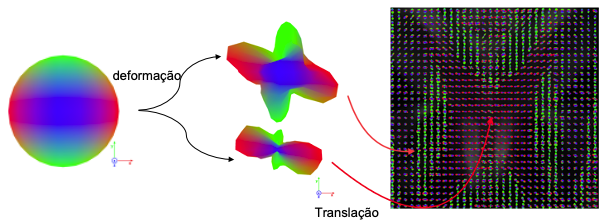
\includegraphics[width=1.0\linewidth, angle=0]{figs/Esquema_Glifo/Renderizacao_multimodal.png}
    \caption{
    Os glifos são gerados a partir da deformação da esfera (à esquerda) e então redimensionados e posicionados na cena (fatia axial).
    }
    \label{fig::esfera_deformada_cena}
\end{figure}

%Em nossa abordagem, a geração da superfície, escalonamento e deslocamento dos glifos ocorre na GPU, a partir de uma malha esférica. %com o deslocamento dos seus $N$ vértices, centrada em $\mathbf{r}$, em função de \textcolor{red}{$\psi_m (\mathbf{r, \mathbf{n}_i}) \mathbf{n}_i$, onde $\mathbf{n}_i$ é o vetor normal à malha esférica no ponto $P_i$ e $\psi (\mathbf{r, \mathbf{n}_i})$ é a função de distribuição de difusão (dODF) min-max normalizada. distribuição de \textit{spin} (SDF) de orientação $\mathbf{n}_i$, seguindo o procedimento apresentado na seção~\ref{sec::glifos_odf}}. \sout{Para uma malha esférica cujo conjunto de vértices é dado por $\{
%P_1,
%P_2, ...,
%P_S
%\}$, o glifo de uma ODF $R(\mathbf{\hat{u}})$ é gerado pelo escalonamento de cada um dos pontos $P_K$ da malha $(1 \leq K \leq S)$ pelo seu respectivo $R(\mathbf{n_K})$, onde $\mathbf{n_K}$ é o vetor unitário com direção e sentido da normal do ponto na esfera em $P_K$.} 

Na CPU, geramos $\boldsymbol{R}(\mathbf{r})$ para todos os \textit{voxels} do volume. Como os espaços de memória da CPU e GPU são distintos, esses dados precisam ser transferidos para GPU. Nesta seção vamos discutir a nossa proposta para representar os dados da geometria dos glifos, malha esférica e a amostragem de $R(\mathbf{r}, \mathbf{\hat{u}})$ em $\boldsymbol{R}(\mathbf{r})$, levando em conta o tráfego entre CPU e GPU e a limitação da memória de vídeo.

% A ODF associada a um \textit{voxel} é tipicamente representada por um conjunto de $N$ amostras de difusão $[
% R(\mathbf{\hat{n}}_1), 
% R(\mathbf{\hat{n}}_2), ...,
% R(\mathbf{\hat{n}}_{N-1}),
% R(\mathbf{\hat{n}}_N)
% ]^T$, onde cada $\mathbf{\hat{n}}_i$ é tem a direção e sentido da normal de cada ponto $ P_i$ de uma malha esférica. O glifo é sintetizado pelo deslocamento de cada ponto $P_i$ pelo seu escalar associado $R(\mathbf{\hat{n}}_i)$. Todas as amostras e ODF são computadas, conforme mostrado no Capítulo \ref{chapter::metodos_hardi} e acessíveis pelos seus respectivos ínndices de \textit{voxel}.

\subsection{Modelagem Multi-resolução}
\label{ssec:modelagem_multiresolucao}

Tomando vantagem da simetria das funções do sinal de difusão em relação aos eixos coordenados \cite{descoteaux2015}, e da propriedade da malha esférica obtida com o procedimento de subdivisões sucessivas de um icosaedro apresentado na Seção \ref{ssec::dominio_esferico} na qual cada vértice presente na malha é acompanhando de sua antípoda, podemos amostrar dODFs usando somente os dados de uma malha semi-esférica.

Propomos categorizar em pontos com subíndice ímpar $\Pi_{impar} = \{P_1$,
$P_3$, ...,
$P_{N-3}$,
$P_{N-1}\}$ nos pontos contidos no hemisfério $\{P(x, y, z) \in \Pi | y > 0 \cup (y = 0 \cap x > 0)\}$, e o restante dos pontos da malha esférica em $\Pi_{par} = \{P_2, P_4, ..., P_{N-2}, P_{N}\}$. Além disso, condicionamos que $P_{2i+2} = -P_{2i+1}$, $(0 \leq i \leq \frac{N-2}{2})$, de forma que os vértices $P_{2i+2}$ e $P_{2i+1}$ sejam vértices antipodais. Assim, para uma malha esférica com $N = 10 \times 4^k + 2$ vértices da tesselação de amostragem, os dados do conjunto de direções $\mathbf{U}_{3\times \frac{N}{2}} = [
\mathbf{n}_1,
\mathbf{n}_3, ..., 
\mathbf{n}_{N-3},
\mathbf{n}_{N-1}
]$, são suficientes para moldar um glifo. Isso nos leva a representar a topologia da malha em separado dos dados de difusão representados por $R(\mathbf{r},\mathbf{n}_i)$. Fig. \ref{fig::direcoes} ilustra a amostragem no conjunto $\mathbf{U}$ a partir dos pontos \sout{na}\textcolor{red}{de uma} semi-esfera. Propomos, ainda, definir cada triângulo da malha esférica usando os índices dos vértices na lista de pontos $\Pi$. Isso facilita o reuso das coordenadas dos pontos na definição de vários triângulos, evitando duplicação de dados na memória. 

Por conta do compromisso entre a qualidade e a eficiência na renderização dos glifos, propomos uma representação multi-resolução para as malhas esféricas de orientações. Pelos testes realizados, \todo{É coerente com o conteúdo do próximo parágrafo? A resolução é adaptativa ou só tem 2 níveis?}recomendamos que a ordem de tesselação para amostragem seja a oitava ($k=3$) ou, no máximo, a décima sexta ($k=4$), implicando em 321 e 1281 amostras de dODFs min-max normalizadas por \textit{voxel}. Valores acima destes computados para todo DWI pode incorrer no uso de uma quantidade proibitiva de memória. Por exemplo, para tesselação de oitava ordem, em que armazenamos os dados em um ponto flutuante de 4 \textit{bytes}, são necessários 1.284 \textit{bytes} por \textit{voxel}, que gera aproximadamente 4.480 \textit{Gigabytes} de memória para um volume de dimensões $145 \times 174 \times 145$ do \textit{Human Connectome Project} \cite{essen2012}.

%\subsection{Geometria base}

%\subsubsection{Considerações iniciais}
%\subsubsection{Multiresolução}

%\sout{As ODFs são amostradas a partir dos vetores normais dos pontos de uma malha base esférica $(\Pi, I)$, onde $\Pi = [P_1, P_2, \dots, P_N]$ consiste num conjunto de pontos não repetidos e o conjunto $I$ são os índices que referenciam os pontos de $\Pi$ para formar os triângulos que sintetizam a malha. Estabelecemos duas condições para a estrutura de dados, nas quais tiramos proveito da simetria de dados das ODFs e para que façamos a malha ser adaptativa para parâmetros de visualização. Estas condições tem impacto direto no tráfego de dados CPU-GPU, conforme discutido na Subseção \ref{ssec::atributos}.}

%\sout{A primeira condição, conforme já discutido no capítulo \ref{chapter::metodos_hardi} na forma de armazenamento de dados da ODF tira vantagem da simetria e armazena os pontos em metade de uma esfera. Propomos que os pontos simétricos em relação aos eixos coordenados de $\Pi$ estejam dispostos de forma consecutiva na memória, i. e. $P_{2i+2} = -P_{2i+1}$, $(0 \leq i \leq \frac{N-2}{2})$, o que nos leva a uma estrutura de dados $\Pi = [P_1, -P_1, P_3, -P_3, \dots, P_{N-3}, -P_{N-3}, P_{N-1}, -P_{N-1}]$.}

Em vista da complexidade em relação à memória, é desejável que a ordem de tesselação seja adaptativa na renderização de glifos, de ordem 1 até 16$^a$ ordem. Propomos que os vértices sejam estruturados numa estrutura linear em $\Pi$. Como os vértices da ordem $2^{t+1}$ $(t < k)$ contêm os vértices da ordem $2^{t}$, propomos anexar, em blocos, os vértices adicionais da ordem $2^{t+1}$ ao bloco dos vértices da ordem $2^t$ como ilustrado na Fig. \ref{fig::icosaedro_blocos}, mantendo a relação de vértices de índices pares e ímpares, ou seja $P_{2i+2} = -P_{2i+1}$. Com isso, garante-se que todos os vértices de uma ordem específica sejam contíguos e que os vértices incrementais de sub-malhas de ordens inferiores estejam organizados em blocos facilmente distinguíveis.

 \begin{figure}[ht]
%\subfigcapskip = -5pt
    \centering
    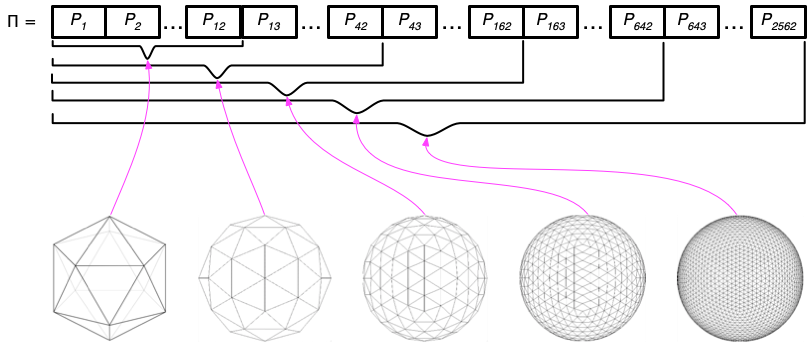
\includegraphics[width=1.0\linewidth, angle=0]{figs/Esquema_Glifo/icosaedro_blocos.png}
    \caption{Ilustração do leiaute em memória do conjunto de vértices $\Pi$ da malha esférica. Da esquerda para direita, as esferas aproximadas pela $1^a$, $2^a$, $4^a$, $8^a$ e $16^a$ ordem de tesselação do icosaedro. A quantidade de vértices de cada malha é obtida de acordo com a Eq. \ref{eq::icosphere_vertices}.}
     \label{fig::icosaedro_blocos}
   %\hspace{1pt}
\end{figure}

%\sout{A segunda condição objetiva fazer a geometria base do glifo ser adaptativa como uma sub-malha da malha esférica base. Seja $k$ o número de sub-malhas de $(\Pi, I)$, onde cada sub-malha é denotada por $(\Pi_i, I_i)$,  $(0 \leq i < k)$, adicionalmente, o número de pontos das sub-malhas é crescente de acordo com os sub-índices, i.e. se $(0 \leq i < j < k)$, implica $|\Pi_j| > |\Pi_i|$. Sugerimos que cada sub-malha $(\Pi_i, I_i)$ seja simétrica em relação a origem e os primeiros $|\Pi_i|$ elementos na estrutura de dados de $\Pi$ corresponda aos elementos de $\Pi_i$. Note que esta condição também implica que, para $i$, $j$ tais $0 \leq i < j < k$, $\Pi_i$ é subconjunto de $\Pi_j$.}

%Adicionalmente, propomos que a alternância de malhas de malhas ocorra em tempo de execução a partir da escolha do conjunto de índices que referenciam os dados de $\Pi$ afim de aproximar esfera pelas tesselações de ordem $0$, $2$, $4$, e assim por diante.

\subsection{Tesselação}
\label{ssec:tesselacao}
%\subsubsection{Formulação da geometria e estruturação de dados}
%\label{sssec::formulação_da_geometria_e_estruturação_de_dados}

%\todo[inline]{Subdivisão sempre com novos triângulos com vértices orientados no sentido anti-horário. \textcolor{green}{Adicionado nesta seção}}

Conforme mencionado na Seção \ref{ssec::dominio_esferico}, escolhemos o conjunto de malhas derivada da $2^k$-ésima ordem de tesselação do icosaedro. O algoritmo para obtermos a tesselação de $2^k$-ésima ordem é um processo iterativo, repetido em $k$ vezes, que se inicia com o icosaedro. Cada triângulo da malha é subdividido em quatro em cada iteração, onde os novos vértices adicionados são computados pela projeção da mediana dos pares de pontos conectados por uma aresta na esfera. Assim, o conjunto de vértices $\Pi$ da $2^k$-ésima ordem contém todos os vértices das iterações anteriores. Adicionalmente, para cada vértice há um vértice antipodal correspondente. O processo de subdivisão de um triângulo está ilustrado na Fig. \ref{fig::icosaedro_faces_2} e um algoritmo para se obter esta categoria de malha pode ser encontrado em \citeonline{luna2012}. Porém, o algoritmo de tesselação do icosaedro apresentado por \citeonline{luna2012} insere muitos vértices repetidos, visto que os pontos medianos computados a cada segmento ocorrem mais de uma vez, dado que dividem duas faces.

%\textcolor{red}{e usa comparações em ponto flutuante para tomadas de decisão, muito sensíveis aos erros de arredondamento.}

Elaboramos um algoritmo de tesselação que realiza inserções não-repetitivas de vértices e que os vértices da ordem $2^{t+1}$ $(t < k)$ sejam adicionados ao bloco de vértices da ordem $2^t$. Além disso, as tomadas de decisão são baseadas em operações inteiras. Para isso, uma lista de arestas é usada. Para cada triângulo da malha esférica, determina-se os pontos médios das suas três arestas para construir os 4 novos triângulos. A lista de arestas é acessada. Se uma aresta já se encontra na lista de arestas, acessa-se o índice do ponto médio da aresta e remova a aresta da lista de arestas. Do contrário, computa-se o ponto médio da aresta, adiciona-se na lista de pontos este ponto médio e o seu ponto antipodal, e insere-se na lista de arestas a aresta com os índices dos seus vértices e o índice do novo ponto médio.

Por uma questão de eficiência na renderização, os triângulos definidos pelo conjunto de índices que referenciam os vértices são \sout{formados}\textcolor{red}{sequencializados} no sentido anti-horário. Assim podemos ativar a funcionalidade de descarte de triângulos não-visíveis (\textit{back-face culling})\sout{, a qual descarta} para remover os polígonos cujos vetores normais formam com o vetor de visão um ângulo maior que 90$^0$ na \textit{pipeline} de renderização. Isso diminui a quantidade de triângulos na renderização dos glifos.

A cada processo de subdivisão, guardamos o conjunto de índices $I_0$, $I_1$, $I_2$, ..., $I_k$ que referenciam $\Pi$ e triangulam a malha esférica de ordem $2^0$, $2^1$, $2^2$, ...,$2^k$, respectivamente. Fig. \ref{fig::icosphere} ilustra malhas esféricas obtida\textcolor{red}{s} com o algoritmo proposto. Por ser uma percentagem pequena do volume total de dados a ser transferido para GPU e ter um impacto significativo no desempenho de renderização, os conjuntos de índices são transferidos para GPU via \textit{buffers} de índices (\textit{index buffers}).
%%%%%%%%%%%%%%%%%%%%%%%%%%%%%%%%%%%%%%%%%%%%%%
\section{Tráfego CPU-GPU}
\label{sec::trafego_cpu_gpu}

Os espaços de memória da CPU e GPU são distintos. Para renderizar glifos ODF sobre um domínio de orientações especificadas por uma malha esférica da ordem 2$^k$, é necessário transferir a malha esférica e as funções  $\mathbf{R}(\mathbf{r})$ das amostras visíveis computadas na CPU para GPU. Embora a qualidade dos glifos renderizados aumenta com a resolução da malha esférica, mostramos na Seção \ref{sec::renderizacao_de_glifos_ODF} que o volume de dados relativos às funções $\mathbf{R}(\mathbf{r})$ cresce exponencialmente com a ordem de tesselação da malha, incorrendo em gargalos na transferência de dados entre CPU--GPU. Abordamos as seguintes soluções para enfrentar o problema de tráfego de dados devido à alta dimensionalidade das dODFs:

%\todo[inline]{d, D são muito usadas para referenciar distância/dimensões, O que acha de usar v no lugar? \textcolor{green}{Feito. Variável trocada tanto em texto, quanto em figura.}}
\begin{enumerate}
    \item identificação do conjunto de $M$ \textit{voxels} visíveis, representados pelo conjunto de coordenadas $V_{3 \times M} = [
\mathbf{v}_1,
\mathbf{v}_2, ..., 
\mathbf{v}_M
]$ sujeitos à renderização;
\item escolha de uma malha esférica a ser deformada dentre as tesselações de ordem $2^1$, $2^2$, ..., $2^k$ do icosaedro em função da área de cobertura das projeções das malhas esféricas sobre o plano de imagem e apenas os dados que deformam a malha escolhida são enviados para GPU;
\item instanciação de uma malha esférica, para que todos glifos sejam gerados a partir de um único modelo de malha; e
\item estruturação dos dados de difusão para que acessos na GPU sejam otimizados.
\end{enumerate}

%Para que possamos utilizar o recurso de instanciação da GPU, transferimos o conjunto de vértices $\Pi = [
%  P_1$,
%$-P_1$,
%$ P_3$,
%$-P_3$,...,
%$ P_{N-1}$,
%$-P_{N-1}]$ para GPU como um atributo a ser replicado a cada instância, em adição ao superconjunto de índices $\{I_1$, $I_2$, ..., $I_k\}$ antes da inicialização da renderização.

%Com os dados das dODF min-max computados e armazenados na CPU; e o conjunto de vértices $\Pi$, e o super conjunto de índices $\{I_1$, $I_2$, ..., $I_k\}$ armazenados na GPU, na Seção \ref{malha_esferica} mostramos o procedimento da escolha malha esférica instanciada e na Seção \ref{ssec::atributos}, mostramos o tráfego de dados CPU-GPU que customizam os glifos em uma requisição de desenho a partir do conjunto de \textit{voxels} visíveis $D = [
%\mathbf{d}_1,
%\mathbf{d}_2, ..., 
%\mathbf{d}_M
%]$.
%\sout{Devido às restrições quanto ao tráfego de dados entre CPU e GPU e à memória em GPUs, três estratégias foram propostas para reduzir o volume de dados: configuração simétrica dos vértices da malha, renderização indexada e instanciação.}

%não só numa demanda proibitiva da memória da GPU e num tempo de processamento excessivo como também 
%\sout{Este procedimento causa uma penalidade em performance devido ao tráfego de dados CPU-GPU devido as mudanças frequentes nas imagens renderizadas em função da interação com o usuário. Assim, nesta seção, apresentamos estratégias para enfrentar esta transferência afim de obter a renderização de forma interativa.
%}

\subsection{Visibilidade e ocupação em tela}
\label{ssec:visibilidade}

 \citeonline{voltoline2021} aplicam o algoritmo de \textit{ray-casting} volumétrico para identificar os \textit{voxels} visíveis. Esse algoritmo consiste em lançar um raio por \textit{pixel} sobre o volume de interesse. O volume é amostrado iterativamente em posições discretas ao longo do caminho, como ilustra a Fig. \ref{fig::raycasting_2d}, até encontrar aqueles que estiverem acima do limiar de ruído pré-especificado. Esses \textit{voxels} correspondem aos \textit{voxels} brancos adjacentes aos \textit{voxels} amarelos na Fig. \ref{fig::raycasting_2d} e são considerados visíveis. Propomos pré-processar o volume b0, carregando-o como textura 3D na GPU de forma análoga ao procedimento apresentado por \citeonline{voltoline2021}. As coordenadas dos primeiros \textit{voxels} visíveis detectados pelo raio são armazenadas numa matriz $\mathscr{M}$ de dimensões da área de \textit{pixels} processados. A partir de $\mathscr{M}$, propomos adotar o algoritmo proposto por \citeonline{voltoline2021} baseado em GPU para obtenção de uma lista sem redundância de $M$ \textit{voxels} visíveis $V_{3 \times M} = [
\mathbf{v}_1,
\mathbf{v}_2, ..., 
\mathbf{v}_M
]$ e a respectiva ocupação de \textit{pixels} em tela. Adicionalmente, a quantidade máxima de \textit{pixels} ocupada por um único \textit{voxel} $\mathbf{v}_i \in V$, $max_p$, também é computado na GPU. Ambos $V$ e $max_p$ são transferidos da GPU para CPU para escolha de resolução e preparação dos dados a serem enviados à GPU para renderização.

%\textcolor{red}{ \sout{Essa matriz é retornada para CPU. Após remover as redundâncias de \textit{voxels} em  $\mathscr{M}$, são transferidas as coordenadas dos \textit{voxels} visíveis para o vetor $V_{3 \times M}$.}}
 
 \begin{figure}[ht]
%\subfigcapskip = -5pt
    \centering
    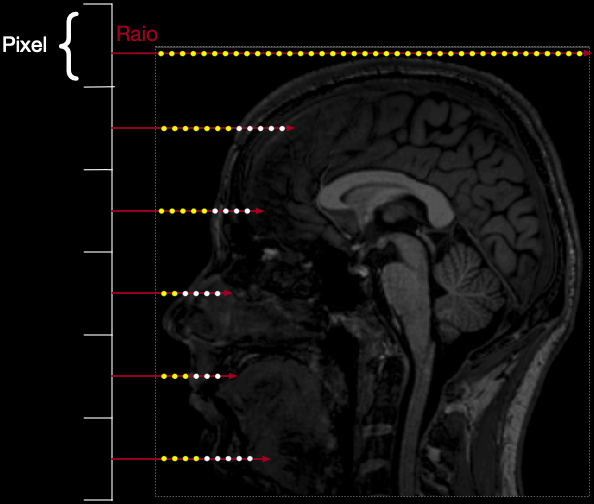
\includegraphics[width=.55\linewidth, angle=0]{figs/Esquema_Glifo/raycasting/raycasting_2d_2.png}
    \caption{Processo de \textit{ray-casting} de um volume MRI. Em vermelho, os raios lançados por \textit{pixel}. Os pontos indicam a amostragem ao longo do raio no volume. Os pontos amarelos indicam pontos externos e os brancos indicam pontos do volume.
     }
     \label{fig::raycasting_2d}
   %\hspace{1pt}
\end{figure}


%Outra estratégia que adotamos é enviar para GPU somente dados de amostras visíveis com uma resolução adaptativa 

%\subsection{Malha Esférica}
\subsection{Nível de Resolução}
\label{malha_esferica}
%\subsection{Escolha automática da geometria base}
%\label{sssec::escolha_automatica_da_geometria_base}

A escolha do nível de resolução da malha esférica para formação dos glifos é baseada no \textit{trade-off} empírico proposto por \citeonline{voltoline2021}, que relaciona a quantidade mínima de triângulos $\tau$ para uma dada cobertura máxima em \textit{pixels}, $max_p$, dos \textit{voxels} sobre a área de imagem:

\begin{equation}
\label{eq::trade_off}
    \frac{max_p}{\tau} < \sqrt{\frac{max_p}{64}}.
\end{equation}
Reajustamos a inequação para estabelecer uma quantidade mínima de triângulos em função de $max_p$
\begin{equation}
\label{eq::trade_off_2}
    \tau > 8\sqrt{max_p}
    .
\end{equation}
% Para explicitarmos a ordem de tesselação na derivação da expressão que escolhe a malha esférica, derivamos a quantidade de triângulos da Eq. \ref{eq::icosphere_triangulos} para $2^t$-ésima ordem de tesselação do icosaedro
%\begin{equation}
%\label{eq::triangulo_icosaordem}
%    \tau = 20\times 4^t
%\end{equation}
Combinando as Eqs. \ref{eq::icosphere_triangulos} e \ref{eq::trade_off_2} e usando o fato de que a quantidade de faces de um icosaedro é $\tau_{min}$ = 20, derivamos uma expressão que relaciona a quantidade de triângulos $\tau$ e $max_p$, onde a subdivisão de ordem um (icosaedro) é mapeado em $max_p = 0$\footnote{Em nossos testes, o conjunto de índices $I_0$ que sintetiza o icosaedro, que tem 12 vértices, não sintetiza os glifos ODF de forma razoável.}:
%\begin{equation}
%\label{eq::maxp_triangulo}
%    \frac{max_p}{\tau - \tau_{min}} = \sqrt{\frac{max_p}{64}},
%\end{equation}
\begin{equation}
\label{eq::maxp_triangulo}
    \tau - \tau_{min} = 8\sqrt{max_p}.
\end{equation}
Substituindo $\tau$ pela Eq. \ref{eq::icosphere_triangulos} temos:
% \begin{equation}
% \label{eq::maxp_order_1}
%     \frac{max_p}{20 \cdot 4^t - 20} = \sqrt{\frac{max_p}{64}}.
% \end{equation}
\begin{equation}
\label{eq::maxp_order_1}
    20 \cdot 4^t - 20 = 8\sqrt{max_p}    .
\end{equation}
Reestruturando a Eq. \ref{eq::maxp_order_1} para que possamos obter a ordem de tesselação $2^t$ em função de $max_p$, \sout{obtemos}\textcolor{red}{chegamos em}:
\begin{equation}
\label{eq::icosa_order}
     t = \lceil \frac{1}{2}\log_2{(\frac{2}{5}\sqrt{max_p} + 1)} \rceil,
\end{equation}
onde o arredondamento de $t$ para o próximo valor inteiro garante que \sout{o \textit{trade-off} d}a Eq. \ref{eq::trade_off} seja satisfeito. Adicionalmente, $t$ é delimitado pela ordem de tesselação utilizada para amostragem dos dados.

%\textcolor{red}{Propomos adotar o algoritmo proposto por \citeonline{voltoline2021} na estimativa de $max_p$. Essencialmente, ele consiste em contabilizar, para cada \textit{voxel} visível $v_j$, a quantidade de entradas das coordenadas de $v_j$ na matriz de \textit{pixels} ${\mathscr M}$ apresentada na seção \ref{ssec:visibilidade}. O valor $max_p$ é o valor máximo de \textit{pixels} ocupados por um único \textit{voxel}.  Adicionalmente, sugerimos realizar a escolha do nível de resolução da malha esférica da tesselação do icosaedro de ordem $2^t$ através da ativação do \textit{index buffer} $I_t$, já carregado na GPU conforme mostra a seção \ref{ssec:tesselacao}. }

%\todo[inline]{Puxei do Cap. 4 para cá ... É mais proposta do que resultados ... Só para você se lembrar e ver se esquecemos de alguma coisa dá para aproveitar em algum ponto do texto ... \textcolor{green}{OK! Eu creio que não...}}
%\textcolor{magenta}{Aplicamos todos os conceitos apresentados até a versão do algoritmo de renderização de ODFs, apresentada na Seção \ref{sec::estrutura_de_dados_para_textura_RGBA}, integramos ao ambiente de visualização multimodal e fizemos as medições de performance conforme descrita na Seção \ref{ssec::performance}, onde utilizamos a tesselação de $8^a$ ordem do icosaedro de forma fixa.
%}

%\textcolor{magenta}{Observe que não conseguimos renderizar os glifos em taxas interativas quando há muitos deles sendo renderizados e para resolver este problema, resolvemos tornar a malha esférica base dos glifos adaptativa. Assim, dividimos este problema em duas partes: (1) como podemos alternar geometrias base para sub-malhas de malha esférica base em tempo de execução; e (2) como podemos diminuir o tráfego de dados para que apenas os dados referentes às sub-malhas sejam enviados à GPU.
%}

%\textcolor{magenta}{Com este objetivo, propomos a segunda condição que restringe o uso da malha esférica base $(\Pi, I)$: $(\Pi, I)$ se torna $(\Pi, I_k)$ e tem $k$ sub-malhas, onde cada sub-malha é denotada por $(\Pi_i, I_i)$,  $(0 \leq i \leq k)$. Adicionalmente, o número de pontos das sub-malhas é crescente de acordo com os sub-índices, i.e. se $(0 \leq i < j < k)$, implica $|\Pi_j| > |\Pi_i|$. Os primeiros $|\Pi_i|$ elementos na estrutura de dados de $\Pi$ corresponde aos elementos de $\Pi_i$. Note que esta condição também implica que, para $i$, $j$ tais $0 \leq i < j < k$, $\Pi_i$ é subconjunto de $\Pi_j$.
%}

%\textcolor{magenta}{Aplicadas estas condições, resolvemos a alternância de malhas esféricas, fazendo com que, no processo de inicialização do algoritmo de renderização, os conjunto de vértices $\Pi$ e os conjunto de índices $I_0$, $I_1$, ..., $I_{k-1}$, $I_k$ sejam carregados na GPU.
%}

%\textcolor{magenta}{Resolvemos o problema de tráfego de dados no envio das amostras, no qual as amostras que deformam a sub-malha esférica de mais baixa resolução são colocadas na parte inicial de $\boldsymbol{R}(\mathbf{r})$, as amostras que deformam a sub-malha esférica de segunda mais baixa resolução, envolve as amostras da primeira e as suas próprias amostras em $\boldsymbol{R(\mathbf{r})}$, e assim por diante.
%}

%\textcolor{magenta}{Sugerimos tesselações do icosaedro de ordem potência de dois para este fim, no qual propomos que os vértices do icosaedro consistam nos primeiros 12 vértices da estrutura de dados, a subdivisão de $2^a$ ordem consista nos 42 primeiros vértices, a subdivisão de $4^a$ ordem consista nos primeiros 162 vértices na estrutura de dados, e assim sucessivamente\footnote{A Eq. \ref{eq::icosphere_vertices} formula a quantidade de vértices em função da ordem de tesselação.}. Adicionalmente, as antípodas estão dispostas de forma consecutiva na memória no conjunto de vértices $\Pi$, assim como nas Seções \ref{sec::otimizacao_da_simetria} e \ref{sec::estrutura_de_dados_para_textura_RGBA}.
%}

%\textcolor{magenta}{A forma que escolhemos para fazer a escolha entre uma destas é baseado na relação heurística de \citeonline{voltoline2021}, que estabelece uma quantidade mínima de triângulos para manutenção de uma boa qualidade visual dos glifos, dado a sua ocupância em \textit{pixels}, que está formulada na Seção %\ref{sssec::formulação_da_geometria_e_estruturação_de_dados}, 
%\ref{malha_esferica}. A quantidade de amostras enviadas à GPU para customizar o glifo das sub-malhas se torna adaptativa, na Seção \ref{sec::renderizacao_de_glifos_ODF}, estruturamos os dados afim de gerar essa adaptabilidade e na Seção \ref{ssec::preparacao_de_dados}, aproveitamos essa estruturação para limitarmos a matriz com somente as amostras que customizam o glifo para a sub-malha escolhida.
%}
% e \ref{sssec::dados_de_odf}.

%Há um procedimento adicional que consiste em setar a quantidade de dados de dODF min-max normalizada por glifo enviado à GPU como uma função de sua quantidade de vértices, o que será discutido mais a frente, na Seção \ref{ssec::atributos}.

%%%%%%%%%%%%%%%%%%%%%%%%%%%%
%$\tau \geq 8\sqrt{max_p}$, ($max_p > 0$). 
%Este \textit{trade-off} estabelece a quantidade mínima de triângulos a ser utilizada na malha que não sacrifica a qualidade de imagem dos glifos. Derivamos uma expressão para a escolha da sub-malha da malha esférica base a partir do caso de igualdade do \textit{trade-off}, no qual substituímos a quantidade de triângulos como uma função da ordem de tesselação do icosaedro e mapeamos o icosaedro para o caso $max_p = 0$. A expressão base está na Eq. \ref{eq::icosa_order_base}:


%\begin{equation}
%\label{eq::icosa_order_base}
%     20\times 4^k - 20\times 4^0 = 8\sqrt{max_p}
%\end{equation}


%\textcolor{magenta}{Derivamos $t$ ($t \leq k$) na Eq. \ref{eq::icosa_order} como a ordem de tesselação do icosaedro escolhida. Como $t$ é inteiro positivo, para satisfazer o \textit{trade-off} de \citeonline{voltoline2021}, arrendondamos o valor para cima.}

%The vertices and amount of triangles and the expression for the vertices and triangles number for each $2^k$ tessellation are in Table \ref{tab::icosahedron_set}. In practice, we recommend $k$ to be equal to 3 or 4, at most. Values of above those may incur a prohibitive amount of memory for pre-computed ODF samples in a DWI.

\subsection{Instanciação}
%\subsection{Atributos}
\label{ssec::atributos}

A instanciação, um recurso disponível a partir da versão 3.1 de OpenGL~\cite{segal2009}, permite que seja transferida uma única malha esférica para GPU e replicá-la quantas vezes necessárias na GPU como diferentes instâncias de dados. Com isso, a quantidade de dados para renderizar $M$ glifos, que antes seria $M \times$ ($N$ vértices da superfície do glifo) e $\frac{N}{2}$ amostras das funções de densidade (de probabilidade), é reduzida a 1 malha e $M$ $\times$ ($\frac{N}{2}$ amostras escalares $R(\mathbf{r}, \mathbf{n}_i)$).

A cada malha instanciada, representada por um conjunto de vértices $\Pi = [
  P_1$,
$-P_1$,
$ P_3$,
$-P_3$,...,
$ P_{N-1}$,
$-P_{N-1}]$ e o índice $t$ do \textit{buffer} de índices $I_t$ de triângulos com vértices indexados, é necessário especificar individualmente (1) um vetor de translação que desloque a malha para o \textit{voxel} correspondente, e (2) as amostras da função $\boldsymbol{R}(\mathbf{r})$ deste \textit{voxel}.

%\subsubsection{Translação}
%\label{ssec::translacao}

%\todo[inline]{Volto a insistir na pergunta: O que você realmente passa da CPU para GPU ... Parece que o vetor de deslocamento é computado. \textcolor{green}{OK! Explicitado no parágrafo}}
Ao invés de enviarmos os vetores de translação, propomos mandar 
as coordenadas $\mathbf{v}(v_x, v_y, v_z)$ dos \textit{voxels} detectados $V_{3 \times M} = [
\mathbf{v}_1,
\mathbf{v}_2, ..., 
\mathbf{v}_M
]$ para GPU e explorar a arquitetura paralela da GPU para efetuar 
os cálculos das coordenadas do vetor
\begin{align}
 \label{eq::translation}
    dx = (v_x + 0.5).spacing_x \nonumber\\
    dy = (v_y + 0.5).spacing_y \\
    dz = (v_z + 0.5).spacing_z \nonumber,
\end{align}
que desloca o glifo centrado na origem para o centro do seu respectivo \textit{voxel} $\mathbf{r}(v_x, v_y, v_z)$ de dimensões $spacing_x$, $spacing_y$ e $spacing_z$.

%Os dados de coordenadas $(v_x, v_y, v_z)$ são recuperados na detecção de \textit{voxels} visíveis (Fig. \ref{fig::vmtk_simplified}) e é copiado da GPU para CPU para preparação dos dados que definem os glifos. Aproveitamos estes dados já armazenados na GPU e os utilizamos como um atributo único por instância, no qual aplicamos Eq. \ref{eq::translation} para computar o seu posicionamento na cena. %Note que os dados de voxel visíveis retornados pelo algoritmo é armazenado em um \textit{buffer} na GPU. Este dado é utilizado diretamente no algoritmo de renderização no \textit{vertex shader} para cômputo do atributo de translação.

%\subsubsection{Preparação de dados para superfície do glifo ODF}
%\label{ssec::preparacao_de_dados}

%Uma dODF min-max normalizada discreta tem dimensão igual à quantidade $N/2$ de vértices na malha esférica tesselada.
As amostras de cada função de dODF min-max normalizada, associada ao \textit{voxel} posicionado em $\mathbf{r}(v_x, v_y, v_z)$, são organizadas em uma coluna $\boldsymbol{R}(\mathbf{r})_{\frac{N}{2} \times 1} = [
R(\mathbf{r}, \mathbf{n}_1)$~
$R(\mathbf{r}, \mathbf{n}_3)$ ~ ... ~
$R(\mathbf{r}, \mathbf{n}_{N-3})$ ~
$R(\mathbf{r}, \mathbf{n}_{N-1})]^T$, onde cada elemento $R(\mathbf{r}, \mathbf{n}_{2i-1})$  na i-ésima posição desloca os pontos $P_{2i-1}$ e o seu ponto antipodal $P_{2i}$ na malha esférica.

%\todo[inline]{Não dá para entender o que você quis destacar no parágrafo abaixo. \textcolor{green}{OK! Falei da organização em blocos}}
Dada a organização em blocos dos dados em $\Pi$ com $N$ vértices, nos quais os vértices das tesselações de ordem $2^{t+1}$ são adicionados em bloco em relação a ordem $2^t$, conforme discutido na Seção \ref{ssec:tesselacao}, $I_t$ referencia os primeiros $W = 10 \times 4^t + 2$ vértices em $\Pi$ para \sout{triangular} \textcolor{red}{um}a tesselação de ordem $2^t$ escolhida (Eq. \ref{eq::icosphere_vertices}), sendo os primeiros $\frac{W}{2}$ elementos de $\boldsymbol{R}(\mathbf{r})$ suficientes para síntese de um glifo.
%\todo[inline]{ Não seria N? \textcolor{green}{N é de amostragem, V é para malha esférica escolhida}}

Para uma malha esférica de ordem $2^t$, geramos na CPU uma matriz $\boldsymbol{\mathscr{R}}_{\frac{W}{2} \times M}$ com todas as amostras nas $\frac{W}{2}$ direções de difusão $\mathbf{n}_j$ \textcolor{red}{de um hemisfério} em cada um dos \textit{M} glifos: 
%\todo[inline]{É bom dar uma boa revisada nas notações da quantidade de pontos em cada glifo ... N, S, V, etc. A contagem de pontos começa com 0 ... O total não está defasado de 1???? \textcolor{green}{Eu resolvo quando introduzo o Vertex\_ID e digo que $P_i$ tem um valor associado Vertex\_ID = i - 1}}

\begin{equation}
\label{eq::R}
\boldsymbol{\mathscr{R}} = 
\begingroup % keep the change local
\setlength\arraycolsep{2pt}
\begin{bmatrix} 
    R(\mathbf{v}_{1}, \mathbf{n}_1) &
    R(\mathbf{v}_{2}, \mathbf{n}_1) & \cdots & 
    R(\mathbf{v}_{M}, \mathbf{n}_1)  \\
    
    R(\mathbf{v}_{1}, \mathbf{n}_3) &
    R(\mathbf{v}_{2}, \mathbf{n}_3) & \cdots & 
    R(\mathbf{v}_{M}, \mathbf{n}_{3}) \\ \vdots & \vdots & \vdots & \vdots  \\
    
    R(\mathbf{v}_{1}, \mathbf{n}_{W-3}) &
    R(\mathbf{v}_{2}, \mathbf{n}_{W-3}) & \cdots & 
    R(\mathbf{v}_{M}, \mathbf{n}_{W-3})  \\
    
    R(\mathbf{v}_{1}, \mathbf{n}_{W-1}) & 
    R(\mathbf{v}_{2}, \mathbf{n}_{W-1}) & \cdots & 
    R(\mathbf{v}_{M}, \mathbf{n}_{W-1})
\end{bmatrix}.
\endgroup
\end{equation}
Limitamos a quantidade de linhas na matriz para $\frac{W}{2}$ ($W \leq N$) visando minimizar o tráfego de dados para apenas escalares que desloquem os vértices da malha para os pontos da malha no nível de resolução escolhido.

\subsection{Coalescência}
\label{ssec::coalescencia}

%\todo[inline]{Vale a pena dar uma boa checada na notação usada para referenciar a posição de um voxel: r, d? \textcolor{green}{Certo! Troquei o d por v em tudo, inclusive figuras.}}

As coordenadas dos vértices \sout{do modelo} de malhas esféricas são passadas como um objeto de \textit{buffer} de vértices (\textit{vertex buffer object}) para GPU. O conjunto de coordenadas dos \textit{voxels} \textcolor{red}{visíveis} detectados $V$ é transferido como um vetor instanciado (\textit{instanced array}). A matriz $\boldsymbol{\mathscr{R}}$ na Eq. \ref{eq::R}, é enviada, por sua vez, para GPU como uma textura 2D de formato RGBA. Cada \textit{texel} no formato RGBA suporta quatro valores. Para otimizarmos acessos aos dados, agrupamos os valores escalares da j-ésima coluna $[
R(\mathbf{v}_{j}, \mathbf{n}_1) ~
R(\mathbf{v}_{j}, \mathbf{n}_3) ~ ... ~
R(\mathbf{v}_{j}, \mathbf{n}_{W-3}) ~
R(\mathbf{v}_{j}, \mathbf{n}_{W-1}) ~
]^T$ de quatro em quatro, como mostrado na Fig. \ref{fig::texelfetch}. Consequentemente, em cada acesso de \textit{texel}, temos quatro valores escalares $
R(\mathbf{v}_{j}, \mathbf{\mathbf{n}}_{8i+1})$ (R), $
R(\mathbf{v}_{j}, \mathbf{\mathbf{n}}_{8i+3})$ (G), $
R(\mathbf{v}_{j}, \mathbf{\mathbf{n}}_{8i+5})$ (B), $
R(\mathbf{v}_{j}, \mathbf{\mathbf{n}}_{8i+7})$ (A) com os quais deslocamos quatro pares de pontos simétricos na malha esférica $P_{8i+1}$, $-P_{8i+1}$, $P_{8i+3}$, $-P_{8i+3}$, $P_{8i+5}$, $-P_{8i+5}$, $P_{8i+7}$, $-P_{8i+7}$ para o j-ésimo glifo visível (também $j$-ésima instância). Desta forma, as dimensões da textura com dados das dODFs é $ \lceil \frac{W/2}{4} \rceil \times M$ e \textcolor{red}{esta textura} tem todas as amostras referentes a uma instância j do modelo de malha armazenadas num espaço contíguo de memória o que facilita múltiplos acessos numa única transação. Se $\frac{W}{2}$ não é divisível por quatro, é necessário inserir mais linhas abaixo da última com valores \textit{dummy}, para que o número de linhas se torne divisível por quatro.

\begin{figure}[ht]
%\subfigcapskip = -5pt
    \centering
    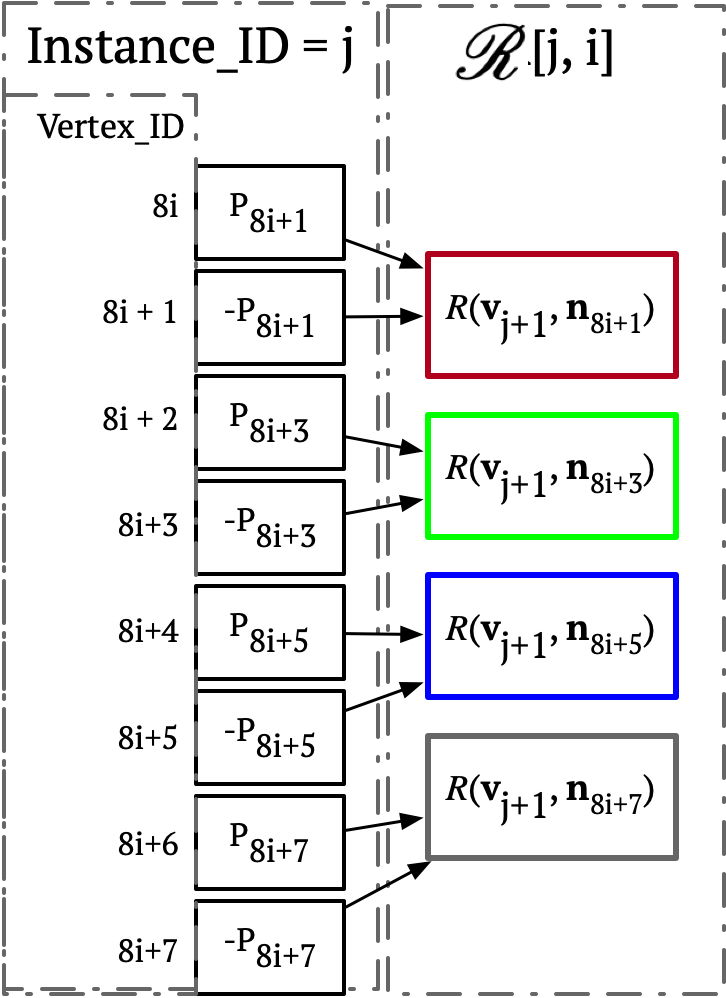
\includegraphics[width=.45\linewidth, angle=0]{figs/Esquema_Glifo/texel_lookup_6.png}
    \caption{Acesso nas componentes RGBA em \textit{texel} de coordenadas (j, i) na textura $\mathscr{R}$. O \textit{texel} é acessado pelas \textit{threads} que processam os vértices de índices 8i, 8i+1, ..., 8i+7 em uma instância $j$. Os blocos de contorno vermelho, azul, verde e cinza ilustram as componentes R, G, B e A do \textit{texel}, respectivamente.}
    \label{fig::texelfetch}
   %\hspace{1pt}
\end{figure}
%%%%%%%%%%%%%%%%%%%%%%%%%%%%%%%%%%%%%%%%%%%%%%
\section{Processamento em GPU}
\label{sec::processamento_GPU}

Por completude, incluímos a renderização dos glifos na GPU. A técnica de renderização é baseada em triângulos (no espaço do objeto), aplicando o tradicional fluxo de renderização programável de OpenGL que requer a programação de um \textit{vertex} e \textit{fragment shaders}. Ativamos funcionalidades de \sout{corte}\textcolor{red}{descarte} de triângulos não-visíveis (\textit{back-face culling}) para ganhos em desempenho e de teste de profundidade (\textit{depth test}) para garantir a correta visibilidade dos glifos.

%\todo[inline]{Visibility Culling e depth map ativados. \textcolor{green}{OK!}}

\subsection{\textit{Vertex Shader}}
\label{ssec::vertex_shader}

%\subsubsection{Acesso dos dados de dODF min-max normalizados}
No \textit{vertex shader}, há dois índices $(i,j)$ que utilizamos para recuperação do escalar $R(\mathbf{v}_j , \mathbf{n}_i)$  que desloca o ponto $P_i$ do j-ésimo glifo na direção do vetor normal da esfera unitária no ponto $P_i$. Utilizamos o índice de instância $Instance\_ID$ para referenciar cada glifo e o índice de vértice $Vertex\_ID$ para cada ponto $P_i \in \Pi$ da malha esférica. Cada instância da malha indexada pelo índice de instância  $Instance\_ID$ é processada com os dados disponíveis no vetor instanciado (\textit{instanced array}) $V$ e em uma coluna da textura $\boldsymbol{\mathscr{R}}$ (Seção \ref{ssec::coalescencia}). Computamos com Eq. \ref{eq::translation} o deslocamento $(dx, dy, dz)$ a partir das coordenadas $\mathbf{v}_j$ do vetor instanciado $V$. Os acessos dos escalares que deslocam os pontos da malha esférica são feitos pela função \textit{texelFetch}, com coordenadas $(Instance\_ID, \lfloor\frac{Vertex\_ID}{8} \rfloor)$\footnote{A notação via coordenadas tem a coluna como primeiro argumento e a linha como segundo argumento.}. O valor retornado consiste em quatro escalares nas componentes R, G, B e A que podem deslocar 4 pares de pontos antipodais na malha. Por convenção, as componentes R, G, B e A são armazenadas como um vetor de quatro elementos, os quais são indexados por 0, 1, 2 e 3, respectivamente. Consequentemente, o escalar que desloca o ponto de índice ímpar para deformação da malha esférica em cada \textit{texel} (R,G,B,A) é acessado pelo índice $\lfloor (Vertex\_ID \mod{8})/2 \rfloor$\footnote{A função em OpenGL para \textit{lookup} em função dos índices de instância e vértice é dada por texelFetch($\boldsymbol{\mathscr{R}}$,ivec2((gl\_VertexID)/8, gl\_InstanceID), 0)[(gl\_VertexID\%8)/2].}. Fig. \ref{fig::texelfetch} ilustra a forma como os acessos são feitos em um único \textit{texel} para oito pontos, 4 de índice ímpar e seus respectivos antipodais de índice par, da malha. 
%\todo{Pela seção 3.3.3, você passa $(dx, dy, dz)$! Aqui dá a entender que você calcula essas coordenadas! \textcolor{green}{Esta versão é a correta e está clareado na Seção que eu menciono isso mais acima.}}

 Tendo posse das coordenadas de translação e do valor $R(\mathbf{v}_j, \mathbf{n}_i)$, sintetizamos a matriz de transformação aplicada a cada ponto $P_i$ da malha instanciada, para a $j$-ésima instância:

%probabilidade de difusão associada à direção $\mathbf{n}_K$ da instância, $R(\mathbf{r}, \mathbf{n}_K)$, a partir da textura $\boldsymbol{\mathscr{R}}$. Isso nos permite construir a matriz de transformação aplicada nas coordenadas $(x_i, y_i, z_i)$ do $Vertex\_ID$.



%\textcolor{red}{No \textit{vertex shader} cada instância de um vértice,  $Vertex\_ID$, da malha esférica unitária é processada com os dados disponíveis no objeto de \textit{buffer} de vértices único por instância ${\mathscr T}$ e na textura $\boldsymbol{\mathscr{R}}$ (Seção \ref{ssec::coalescencia}). Com o par $(Instance\_ID, \lfloor\frac{Vertex\_ID}{8} \rfloor)$, obtém-se com uso da função \textit{texelFetch} a probabilidade de difusão associada à direção $\mathbf{n}_K$ da instância, $R(\mathbf{r}, \mathbf{n}_K)$, a partir da textura $\boldsymbol{\mathscr{R}}$. Isso nos permite construir a matriz de transformação aplicada nas coordenadas $(x_i, y_i, z_i)$ do $Vertex\_ID$.}

%Os dados das dODFs min-max normalizadas são acessados no \textit{vertex shader}, quando cada glifo da $j$-ésima instância é processada. Utilizamos a variável $Vertex\_ID$ presente no \textit{shader} e que contém um índice inteiro
%para o vértice processado. Cada $P_i \in \Pi$ é associado a $Vertex\_ID = i-1$.

%Os \textit{texels} na coluna $j$ e índice de linha $K = \lfloor\frac{Vertex\_ID}{8} \rfloor$ são acessados para deslocar oito pontos. Usamos a função \textit{texelFetch} para acessar diretamente a textura de ODF utilizando coordenadas não-normalizadas $(j, \lfloor\frac{Vertex\_ID}{8} \rfloor)$. O valor utilizado para \textit{lookup} da componente  para deslocar o seu respectivo ponto na malha esférica no \textit{vertex shader} é acessível pela análise do resto da divisão por oito do $Vertex\_ID$, como ilustrado na Fig. \ref{fig::texelfetch}. Adicionalmente, utilizando a notação via colchetes, onde as componentes R, G, B e A são mapeados nos índices 0, 1, 2 e 3, respectivamente, o escalar de deformação do glifo pode ser mapeado por $\lfloor (Vertex\_ID \mod{8})/2 \rfloor$\footnote{A função em OpenGL para \textit{lookup} em função dos índices de instância e vértice é dada por texelFetch($\boldsymbol{\mathscr{R}}$,ivec2((gl\_VertexID)/8, gl\_InstanceID), 0)[(gl\_VertexID\%8)/2]}.


%\subsubsection{Transformações geométricas}

%Podemos sintetizar as transformações aplicadas a cada vértice $P_K$ em coordenadas homogêneas na $j$-ésima instância por uma multiplicação matricial por uma matriz $G_{Kj}$:
%\todo[inline]{Substituir por $P_i$.}
\begin{equation}
    G_{ij} = \mathbf{M_{vp}}\cdot M_D \cdot M_S \cdot M_{ij},
\end{equation}
onde $M_{ij}$ desloca o ponto da malha esférica ao longo do vetor normal do ponto: 
\begin{equation}
\label{eq::dodf}
    M_{ij} = \begin{bmatrix} 
   \mbox{\small $R( \mathbf{v}_j, \mathbf{n}_i)$} & 0 & 0 & 0 \\
    0 & \mbox{\small $R( \mathbf{v}_j, \mathbf{n}_i)$}  & 0 & 0 \\
    0 & 0 & \mbox{\small $R( \mathbf{v}_j, \mathbf{n}_i)$}  & 0 \\
    0 & 0 & 0 & 1 \\
\end{bmatrix},
\end{equation}
$M_{S}$ \sout{dimensiona}\textcolor{red}{muda o fator de escala d}o glifo para caber em seu respectivo \textit{voxel}
\begin{equation}
    M_{S} = \begin{bmatrix} 
    \frac{mS}{2} & 0             & 0            & 0 \\
    0            & \frac{mS}{2} & 0            & 0 \\
    0            & 0             & \frac{mS}{2} & 0 \\
    0            & 0             & 0            & 1 \\
\end{bmatrix},
\end{equation}
sendo $mS=min(spacing_x , spacing_y , spacing_z)$,
$M_{D}$ \sout{translada}\textcolor{red}{desloca} o glifo para o centro do seu respectivo \textit{voxel}:
\begin{equation}
\label{eq::displace}
    M_{D} = \begin{bmatrix} 
    1 & 0 & 0 & dx \\
    0 & 1 & 0 & dy \\
    0 & 0 & 1 & dz \\
    0 & 0 & 0 & 1 \\
\end{bmatrix},
\end{equation}
e $\mathbf{M_{vp}}$ é a matriz \textit{view-projection} que configura parâmetros de visão e projeção.



%\textcolor{magenta}{Note que, utilizando a notação via colchetes, onde as componentes R, G, B e A são mapeados nos índices  respectivamente, o escalar de deformação do glifo pode ser mapeado por .}

\subsection{\textit{Fragment Shader}}

No \textit{fragment shader} fazemos a definição de cor de cada \textcolor{red}{\textit{pixel}}. Enviamos os valores absolutos das três componentes dos vértices da esfera unitária instanciada $(|P_x|, |P_y|, |P_z|)$ a partir do \textit{vertex shader} e atribuímos este valor a cor do fragmento, conforme Eq. \ref{eq::cor_glifo}.


\section{Renderização multimodal de glifos ODF}
\label{sec::superquadricas}

Nesta seção, descrevemos uma forma de integração do algoritmo proposto no 
ambiente de visualização multimodal para exames imagiológicos desenvolvido no Laboratório de Engenharia de Computação e Controle Industrial da Faculdade de Engenharia Elétrica e de Computação. O aplicativo é conhecido por \textit{Visual Manipulation Toolkit for NeuroImages} (VMTK-Neuro) \cite{VMTKNeuro}.

Neste ambiente está integrada a renderização multimodal dos glifos superquádricos. O algoritmo consiste de três estágios: (1) co-registro do volume b0 de DWI e do volume anatômico  \cite{ting2014}; (2) detecção dos \textit{voxels} visíveis do volume b0 e estimativa da cobertura máxima da projeção dos \textit{voxels} em \textit{pixels}, $max_p$ \cite{voltoline2021}; (3) renderização do volume anatômico pela técnica \textit{ray-casting} (Fig. \ref{fig::raycasting_2d}) \cite{kruger2003} e renderização, na resolução estimada, dos glifos nos respectivos \textit{voxels} visíveis pela técnica de rasterização do fluxo padrão de OpenGL.
%\todo[inline]{\textcolor{green}{Não entendi o que tenho que referenciar?! Do OpenGL?}}

O fluxo de controle foi adaptado para renderização multimodal de glifos ODF. Fig. \ref{fig::vmtk_simplified} apresenta o diagrama de blocos da renderização multimodal dos glifos ODF, adaptada. O \textit{setup} dos dados de ODF está descrito na Seção \ref{sec::renderizacao_de_glifos_ODF} e a renderização de glifos ODF está detalhada na Seção \ref{sec::processamento_GPU}. Os vértices de um modelo de malha esférica (base) são gerados na CPU e transferidos para GPU (Seção \ref{sec::trafego_cpu_gpu}). Na GPU eles são replicados em tantas instâncias quanto a quantidade de \textit{voxels} visíveis. As $k$ listas, $I_1$, $I_2$, $\cdots$, $I_k$, de triângulos definidos por vértices indexados para malhas de diferentes níveis de resolução são também construídas na CPU e transferidas para GPU uma única vez. Adicionalmente, outros parâmetros como espaçamento $(spacing_x, spacing_y, spacing_z)$ entre duas amostras no volume $b0$, o fator de escala a ser aplicado sobre os glifos $mS/2$ são enviados uma vez como variáveis uniformes. A cada requisição de desenho, as amostras de $\boldsymbol{R}(\mathbf{v}_1)$, $\boldsymbol{R}(\mathbf{v}_2)$, ...,
$\boldsymbol{R}(\mathbf{v}_M)$ definidas para os \textit{voxels} \sout{detectados}\textcolor{red}[visíveis] são transferidos para GPU como textura. Para diminuição de tráfego de dados, utilizamos as coordenadas dos \textit{voxels} já computadas na GPU como um vetor instanciado (\textit{instanced array}) (Seção \ref{ssec::atributos}).


%O conjunto de vértices é enviado como um , o super-conjunto de \textcolor{red}{As amostras de dODFs definidas para os \textit{voxels} detectados são transferidos para GPU como textura, e os vetores de translação são enviados como  consistem em objetos  enquanto outros parâmetros como espaçamentos  entre duas amostras do volume b0 e o fator de escala a ser aplicado sobre glifos $mS$ e os \todo{Na memória de textura?}vetores de translação são transferidos como variáveis dos registradores.}  

%fig::flowchart_vmtk_hardi


%\todo[inline]{A legenda da Figura 3.4 é um texto de uma seção e não uma legenda! Note que mudei a letra D para V no texto. Faltaram os vetores de translação \textcolor{green}{Texto resolvido. Sobre a translação, eu aproveito os dados que já estão na GPU, e acabo não transmitindo de volta. Eu os utilizo como vbo único por instância}}

\begin{figure}[ht]
    \centering {
    %\rule{6cm}{3cm}
    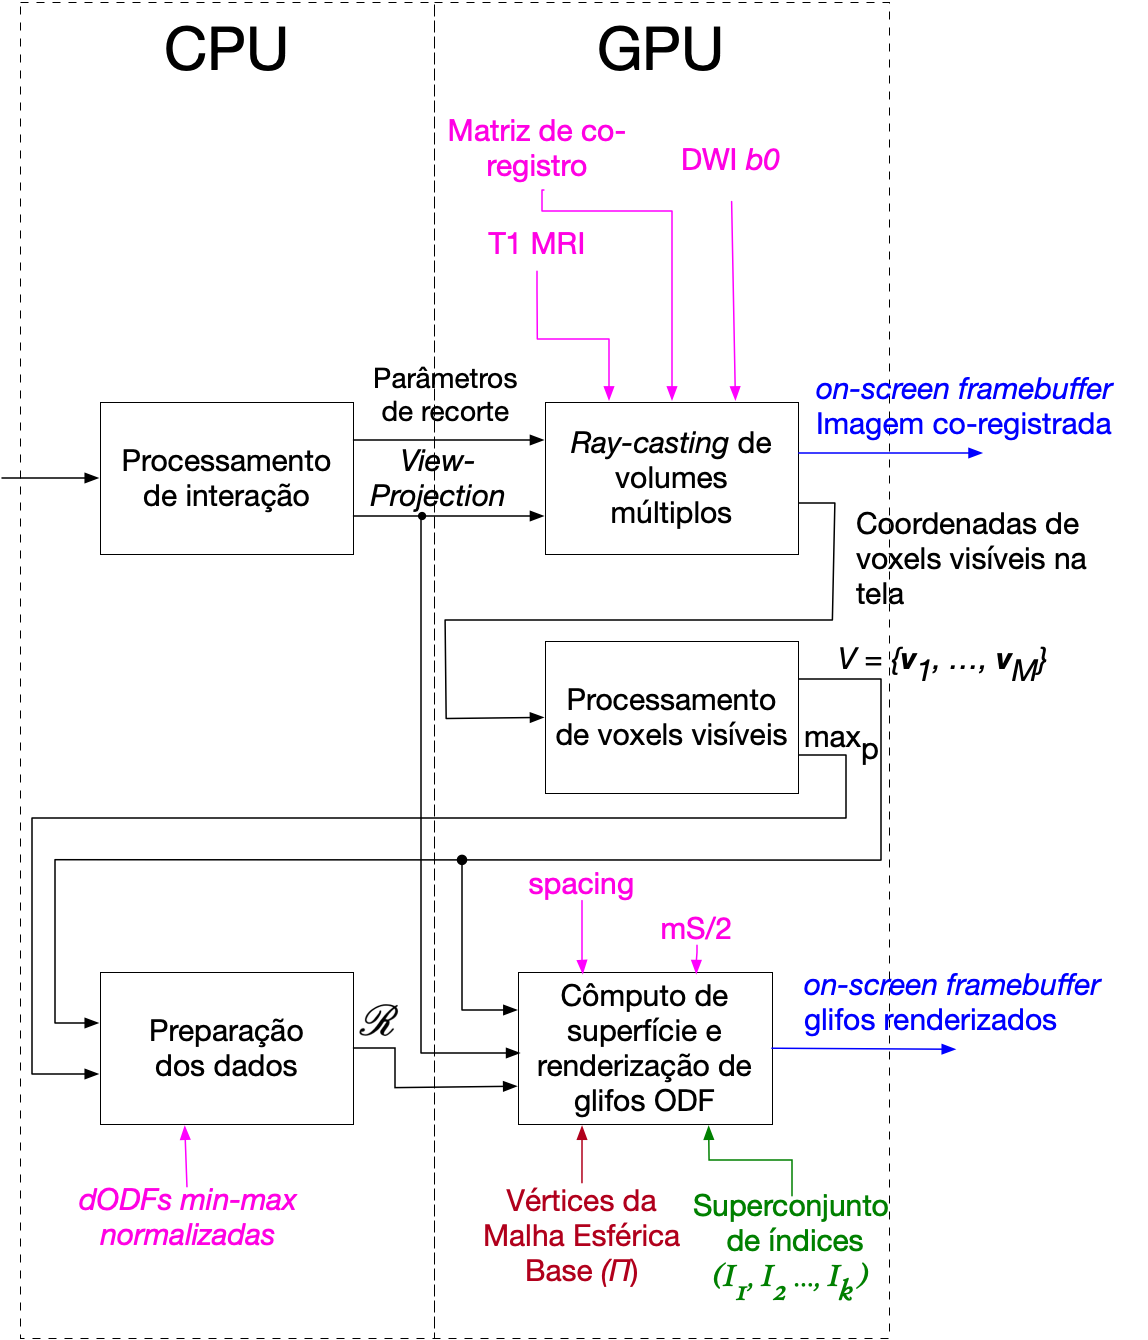
\includegraphics[width=.7\linewidth, angle=0]{figs/Esquema_Glifo/fluxograma_glifos_VMTK.png}
    \caption{
    Renderização multimodal para glifos ODF. A cor azul representa a saída a ser desenhada, armazenada no \textit{framebuffer} (FB); a cor magenta se refere a dados pré-computados. As setas pretas indicam entrada e saída de dados computados nos módulos apresentados.
    }
   \label{fig::vmtk_simplified}
    }
 \end{figure}
 
 Em \sout{todas as interações}\textcolor{red}{cada interação} com o usuário, todo o fluxo de controle ilustrado na Fig. \ref{fig::vmtk_simplified} é executado. Categorizamos as interações em dois conjuntos, conforme ilustrado na Fig. \ref{fig::vmtk_interacao}: edição de parâmetros de \sout{visualização (\textit{viewing parameters})} \textcolor{red}{rotação} e de recorte \textcolor{red}{do volume anatômico}. Os parâmetros \sout{visualização}\textcolor{red}{de rotação} são sintetizados na CPU \sout{na matriz \textit{view-projection} e enviados à GPU  e se referem à transformação da cena para o espaço da câmera, movimentada pelo usuário} \textcolor{red}{em ângulos de rotação e enviados à GPU como parte da matriz \textit{view-projection}}. Os parâmetros de recorte configuram seis cortes aplicados no volume \textcolor{red}{anatômico} para visualização do seu interior e estes parâmetros se referem a \sout{um par de cada um dos planos anatômicos}\textcolor{red}{pares de planos nos eixos anatômicaos, isto é} \sout{. Os planos consistem no par de} planos axiais \textit{top} e \textit{bottom}; \sout{nos} sagitais \textit{right} e \textit{left}; e \sout{nos} coronais \textit{front} e \textit{back}\textcolor{red}{, que delimitam o sub-espaço do volume anatômico a ser enviado à GPU}.
 
 % em recortar o objeto para visualização da fatia o visualização do objeto de configuração de renderização obtidos com a edição são computados na CPU e enviados à GPU. 

 \begin{figure}[htb]
    \centering
    \subfloat[Ponto inicial de renderização.] {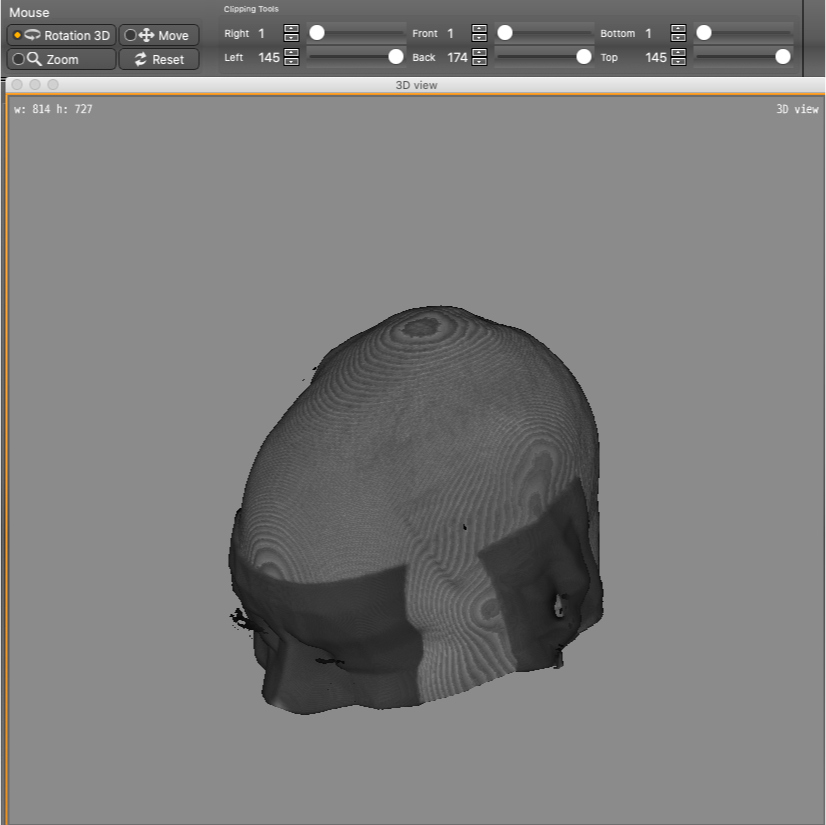
\includegraphics[width=.47\linewidth,  angle=0]{figs/Esquema_Glifo/raycasting/ilustracao_interacao/vmtk_inicial.png}
    \label{fig::vmtk_interacao_inicial}
    }
     \subfloat[Rotação (edição de parâmetros de visualização).]{\makebox[1.\width]
     {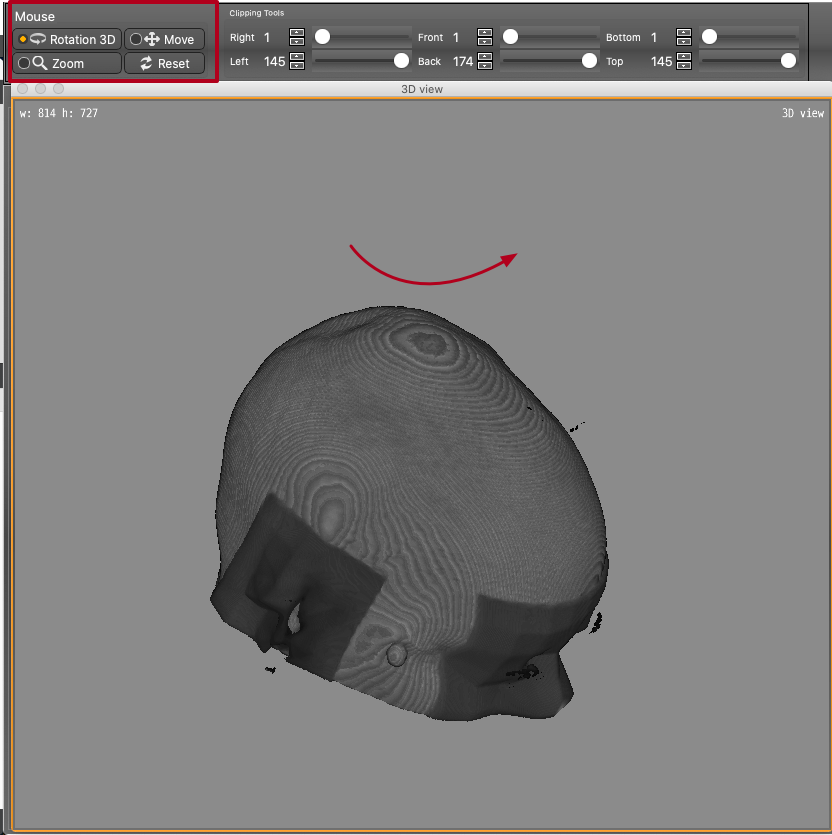
\includegraphics[width=.47\linewidth,  angle=0]{figs/Esquema_Glifo/raycasting/ilustracao_interacao/vmtk_rotacao.png}
    \label{fig::vmtk_interacao_rotacao}
    }
    }
    \\
     \subfloat[Redição de parâmetros de recorte.]{\makebox[1.\width]
     {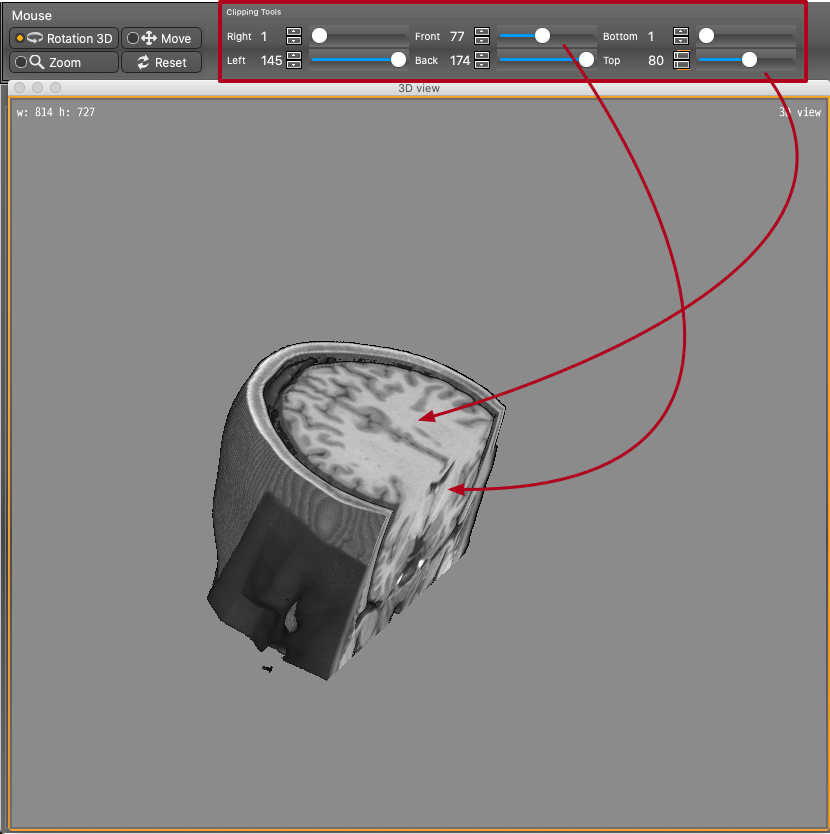
\includegraphics[width=.47\linewidth,  angle=0]{figs/Esquema_Glifo/raycasting/ilustracao_interacao/vmtk_clip.png}
    \label{fig::vmtk_interacao_clip}
    }
    }
    \caption{Interações do usuário com o VMTK-Neuro para visualização de um volume ponderado em T1 de MRI. A Fig. \ref{fig::vmtk_interacao_rotacao} ilustra uma rotação feita em relação à imagem gerada na Fig. \ref{fig::vmtk_interacao_inicial}, e Fig. \ref{fig::vmtk_interacao_clip} ilustra um recorte efetuado na Fig. \ref{fig::vmtk_interacao_rotacao}. Volume do repositório \textit{Wu-Minn Human Connectome Project Retest} do \textit{Connectome Project Consortium} \cite{essen2012}.
    }
    \label{fig::vmtk_interacao}
\end{figure}
 
 %!!VERIFICAR TEXTO DAS INTERAÇÕES
%Toda a \textit{pipeline} de renderização no \textit{VMTK-Neuro} é executada para todas as interações do usuário, que são sintetizados nos parâmetros de renderização e da matriz \textit{View-Projection}. A matriz \textit{View-Projection} sintetiza parâmetros de rotação da cena, mudança de fator de escala e deslocamento na cena. Os parâmetros de renderização que consistem na seleção de fatias, que por sua vez modulam a geometria \textit{proxy}\footnote{Geometria \textit{proxy} é a geometria que contém o objeto a ser visualizado via \textit{ray-casting}}.

%\subsection{Ray-casting de volumes múltiplos}

%No ambiente, a visualização se dá em torno de ambos volumes DWI $b0$ e MRI anatômico ponderado em T1. Os volumes são co-registrados a partir de uma matriz de co-registro rígido \cite{ting2014}, tendo $b0$ como referência e o MRI T1 como flutuante \cite{voltoline2021}. Os volumes transferidos à GPU e são renderizados via \textit{ray-casting} \cite{kruger2003}, que é uma técnica bem estabelecida para renderização de sinais de MRI.

%\sout{No \textit{ray-casting}, um raio é lançado por \textit{pixel} sobre o volume de interesse. O processo é iterativo, no qual o raio é amostrado em posições discretas ao longo do caminho no qual o nível de cinza é computado através dos sinais de MRI do volume.}

%Para cômputo do nível de cinza, há dois atributos gráficos extraídos do volume, que consistem no nível de cinza por \textit{voxel} $C_{src}$ e opacidade $\alpha_{src}$. Ao longo do raio estes atributos são acumulados a partir dos dados da iteração anterior, afim de computar um tom de cinza $C_{dst}$ e opacidade $\alpha_{dst}$, que são inicialmente zerados:

%\begin{equation}
%    C_{dst} = C_{dst} + (1-\alpha_{dst})C_{src},
%\end{equation}
%\begin{equation}
%    \alpha_{dst} = \alpha_{dst} + (1-\alpha_{dst})\alpha_{src}.
%\end{equation}

%O processo iterativo é terminado quando acabam as amostras do volume para contribuição na cor do \textit{pixel}, ou quando $\alpha_{dst}$ atinge um limiar de superfície opaca $\alpha_{max}$. O nível de cinza do fragmento e opacidade são definidos como $C_{dst}$ e $\alpha_{dst}$. Fig. \ref{fig::ilustracao_raycasting} ilustra o algoritmo.

%\begin{figure}[ht]
%\centering
%\captionsetup[subfloat]{farskip=0pt,nearskip=0pt}
%\centering
%   \subfloat[Em vermelho, os raios lançados por pixel. Os pontos indicam o ponto de amostragem do raio no volume, onde o valor do \textit{voxel} $C_{src}$ e $\alpha_{src}$ são extraídos para cômputo de $C_{dst}$ e $\alpha_{dst}$. Os pontos amarelos indicam espaço vazio e os brancos indicam pontos do volume. Por simplicidade, ilustramos para apenas seis \textit{pixels}, enquanto a quantidade real para o plano é dado pelo comprimento da imagem em \ref{fig::raycasting_3d}.
%    ]{\makebox[1.7\width]{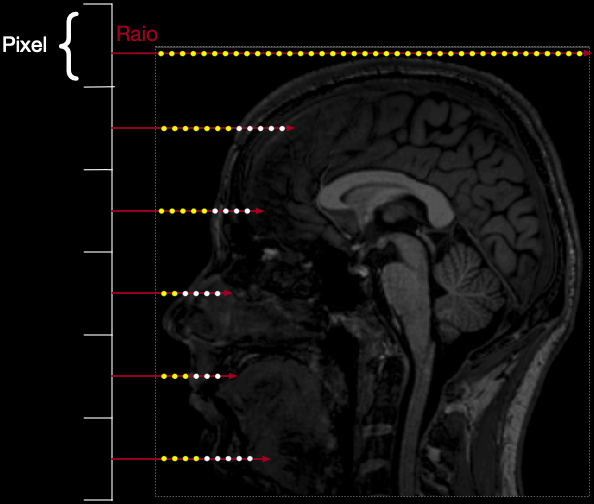
\includegraphics[width=.55\linewidth, angle=0]{figs/Esquema_Glifo/raycasting/raycasting_2d_2.png}
%    \label{fig::raycasting_2d}
%    }
%    }
%    \\
%    \hspace{1em}
%    \subfloat[Volume 3D renderizado via \textit{ray-casting}] {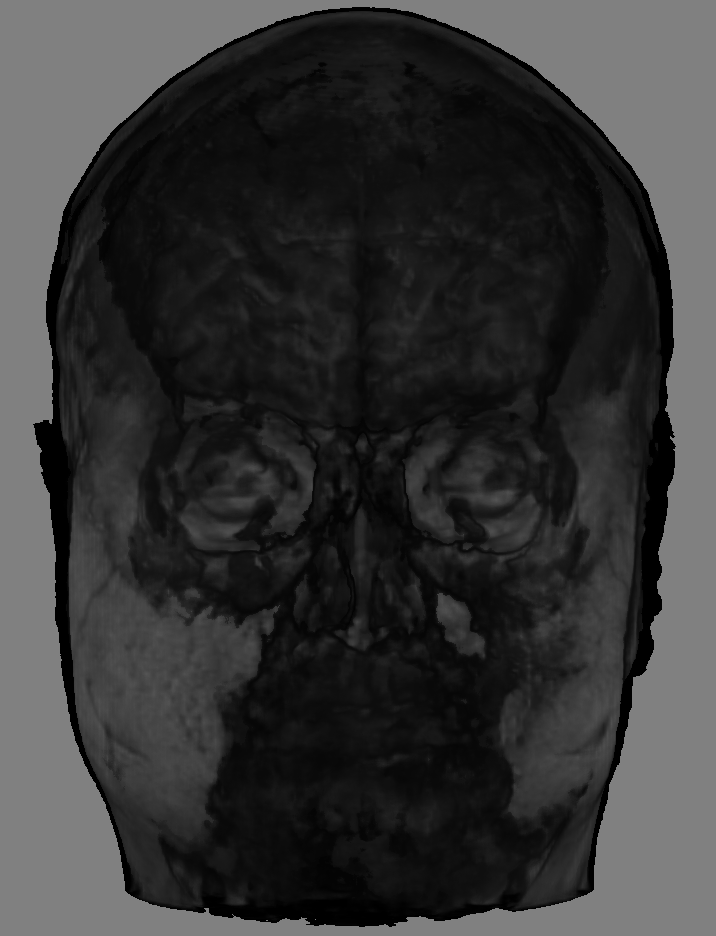
\includegraphics[width=.37\linewidth, angle=0]{figs/Esquema_Glifo/raycasting/raycasting_3d.png}
%    \label{fig::raycasting_3d}
%    }
%     \caption{Ilustração do processo de \textit{ray-casting} de um volume MRI. Fig. \ref{fig::raycasting_2d} ilustra o \textit{ray-casting} para os \textit{pixels} situados em um plano ortogonal à Fig. \ref{fig::raycasting_3d} na coluna central da visualização 3D.}
%    \label{fig::ilustracao_raycasting}
%\end{figure}

%No \textit{ray-casting} de volumes múltiplos, a cor é determinada pela soma ponderada entre dois volumes, que são co-registrados afim de estarem no mesmo espaço tridimensional.

%No processo de renderização na GPU dos volumes co-registrados, uma matriz com as dimensões da janela de renderização é definida onde os elementos de coordenada  $(x, y)$ armazenam as coordenadas $(v_x, v_y, v_z)$ do primeiro \textit{voxel} visível atingindo pelo raio no algoritmo de \textit{ray-casting}.

%\subsection{Processamento de \textit{voxels} visíveis}


%\subsection{Renderização de glifos ODF}

%Enviamos os conjunto $D = [
%\mathbf{d}_1,
%\mathbf{d}_2, ..., 
%\mathbf{d}_M
%]$ de \textit{voxels} visíveis detectados e $max_p$ da GPU para a CPU no qual preparamos os dados pré-computados que sintetizam os glifos a serem renderizados. Enviamos estes dados à GPU para que cada glifo seja sintetizado e renderizado de forma sobreposta ao seu respectivo \textit{voxel}.

%O procedimento de pré-computo, a preparação dos dados que sintetizam os glifos, bem como o processamento da GPU para renderização serão apresentados nas Seções \ref{malha_esferica}, \ref{sec::trafego_cpu_gpu} e \ref{sec::processamento_GPU}.

 %que cada um ocupa são computados, cujo algoritmo foi proposto por \citeonline{voltoline2021}





%Para manter a compatibilidade do algoritmo com o Mac OSX, cuja versão máxima suportada do OpenGL é 4.1, eles desdobraram o algoritmo para estimação de cobertura máxima de \textit{pixels} para os glifos de um passo, onde a implementação é feita no \textit{compute shader} em um algoritmo de quatro passos, envolvendo \textit{vertex, geometry} e \textit{fragment shaders} baseados em rasterização. Para evitar transferência de dados entre CPU e GPU entre passos, o \textit{transform feedback buffer} foi aplicado. Adicionalmente, eles mostraram a utilização do mecanismo de \textit{additive blending} para obtenção do número máximo de \textit{pixels} ($max_p$), no qual o \textit{voxel} é projetado em um volume \textit{ray-casted}. Baseado em $max_p$, eles estabelecem uma heurística para estimação da resolução da malha.


%\citeonline{voltoline2021} propuseram um algoritmo de renderização multimodal de glifos superquádricos sobre o seu respectivo MRI anatômico ponderado em T1. O volume $b0$, seu respectivo MRI T1 e a matriz rígida que co-registra ambos os volumes  são enviadas à GPU.







%Através de $max_p$, um \textit{tessellation shader} é acionado para gerar o \textit{skeleton} base dos superquádricos, no qual eles utilizam o comando renderização indireta por instâncias para desenhá-los com uma chamada desenho. Provendo a parâmetros particulares a cada \textit{voxel} que definem cada superquádrico, em cada instância o \textit{skeleton} é customizado para gerar o glifo e é posicionado em seu respectivo \textit{voxel} no espaço do volume.



%\section{Inicialização do algoritmo}
%\label{sec::inicialização_do_algoritmo}

%Após a tesselação do icosaedro e antes da renderização dos glifos, definimos o domínio de amostragem das dODFs min-max normalizadas $\mathbf{U} = [
%\mathbf{n}_1$,
%$\mathbf{n}_3$, ...
%$\mathbf{n}_{N-3}$,
%$\mathbf{n}_{N-1}]$, onde $\mathbf{n}_i$ é o vetor unitário com direção e sentido de $P_i \in \Pi_{impar}$
%e as computamos para todos os \textit{voxels} da aquisição DWI, como mostrado na Seção \ref{sec::gqi} e \ref{sec::vis_dODFs} e as mantemos na CPU.

%Pela alta dimensionalidade das dODFs min-max normalizadas $\boldsymbol{R}(\mathbf{r})$, as mantemos na CPU, e em tempo de execução da renderização, as enviamos sob demanda para GPU para definição das superfícies dos glifos, o que potencialmente gera um elevado tráfego de dados no processo, que afeta a performance e interatividade da renderização, nos quais discutimos na Seção \ref{sec::trafego_cpu_gpu}.

%Para ajustar o tamanho dos glifos ao tamanho dos seus respectivos \textit{voxels}, redimensionamos os glifos com base nos espaçamentos entre \textit{voxels} da aquisição \cite{voltoline2021} com base em um fator de escala dado por $mS/2$, no qual:
%\begin{equation}
%    mS = min(spacing_x, spacing_y, spacing_z),
%\end{equation}
%onde  $spacing_x$, $spacing_y$, $spacing_z$ é o espaço entre duas amostras adjacentes nos eixos x, y e z, respectivamente. Enviamos $mS/2$ para GPU como uma variável uniforme.



%potencialmente pode afetar a performance do algoritmo de renderização devido à elevada quantidade de dados.


%\begin{figure}[htb]
%    \centering
%    %\rule{6cm}{3cm}
%    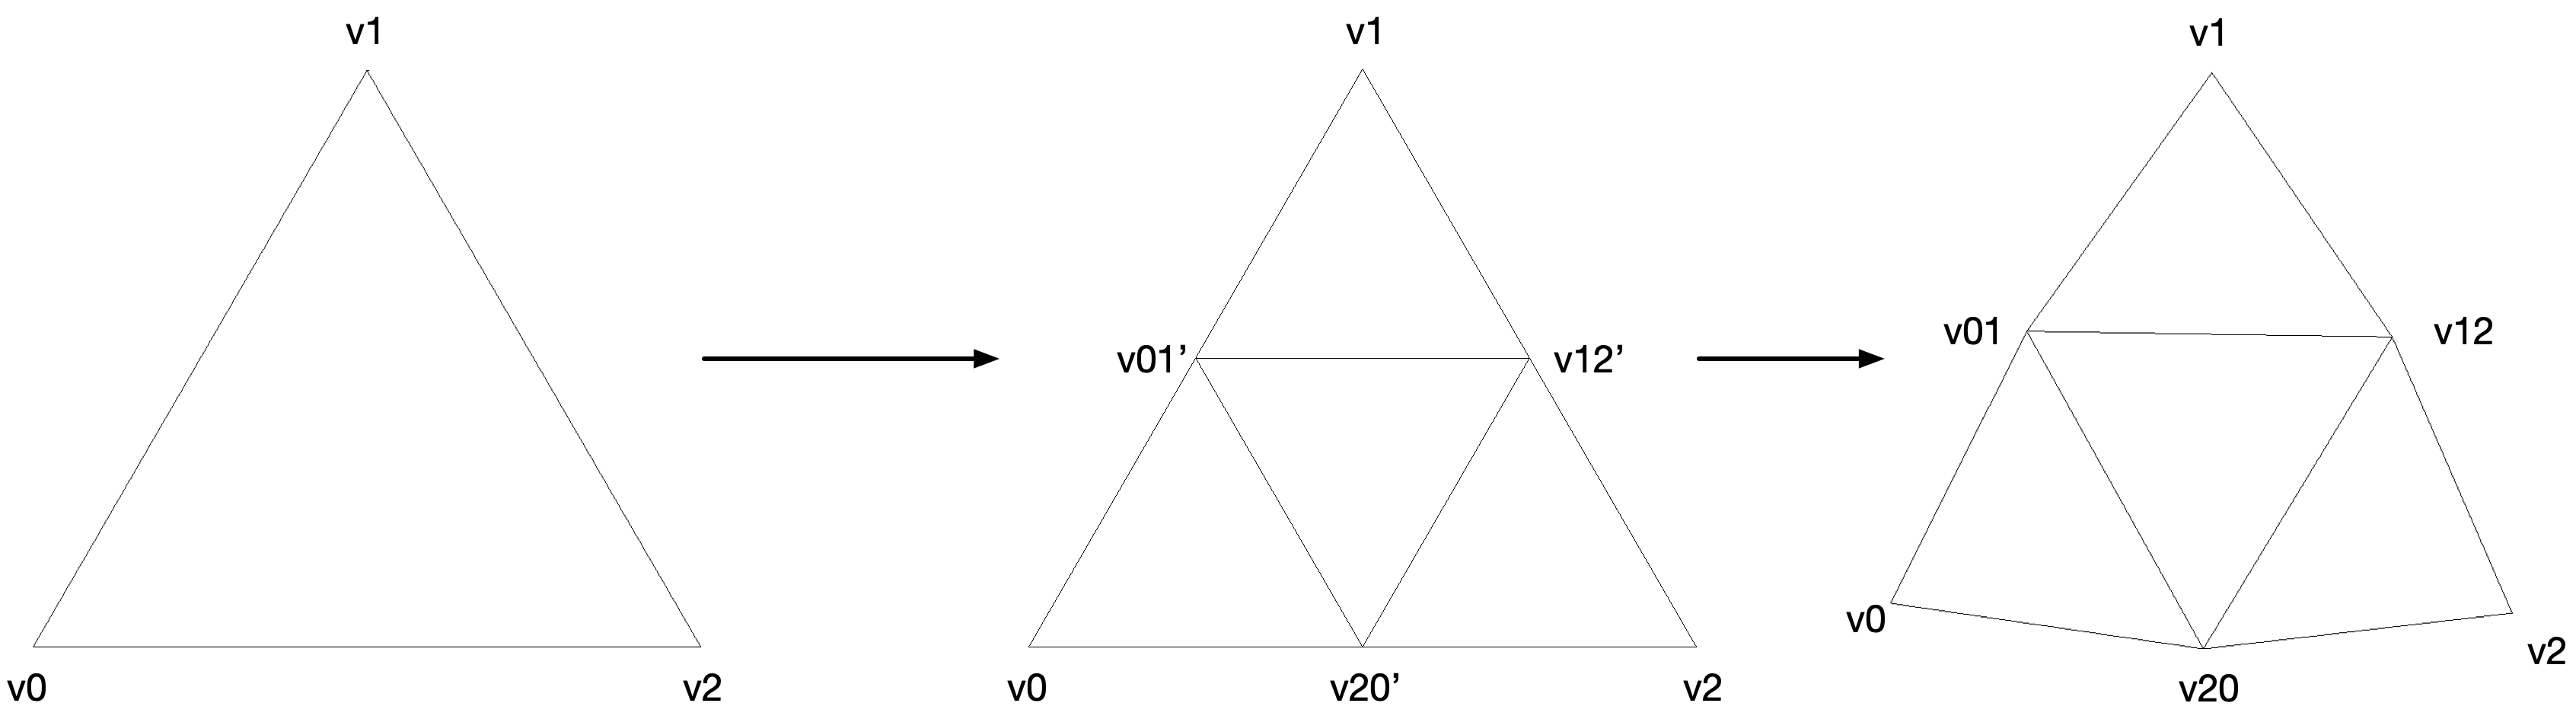
\includegraphics[width=1.0\linewidth, angle=0]{figs/Esquema_Glifo/ico_subdivision.png}
%    \caption{
%    Subdivisão de um triângulo para formar quatro na formação da malha esférica a partir da tesselação de $2^k$-ésima ordem a partir da partir da $2^{k-1}$-ésima. O triangulo formado pelos vértices $v0$, $v1$ e $v2$ é subdividido em quatro, onde as medianas  $v01'$, $v12'$ e $v20'$ são computadas e suas respectivas projeções na esfera $v01$, $v12$ e $v20$ são adicionados ao conjunto de vértices.
%    }
%    \label{fig::triangle_icosahedron}
%\end{figure}

%\sout{Assim como mencionado no capítulo \ref{chapter::metodos_hardi}, por questões de memória, recomendamos k = 3, ou no máximo 4. Assim, formulamos a estrutura de dados que satisfaz as duas condições que estabelecemos a princípio, e é tal que os primeiros 12 elementos correspondem aos vértices do icosaedro, os 42 primeiros elementos correspondem aos vértices da $2^a$ ordem de tesselação, os 162 primeiros elementos correspondem a $4^a$ ordem de tesselação, os primeiros 642 elementos correspondam a $8^{a}$ ordem de tesselação, e, adicionalmente, os pontos simétricos são agrupados em sequencia na memória.}

%\sout{A estrutura de dados $\Pi$, e $I$, além dos índices que triangulam todas as sub-malhas, contidos ao superconjunto $\mathbf{I}$ no Algoritmo \ref{alg::setIcosahedroBase}, são enviados à GPU uma vez. Uma vez que os dados estão na GPU, e visando eficiência no processamento, sem comprometer a qualidade visual, escolhemos adaptativamente a geometria base entre estas malhas por um procedimento heurístico computado em tempo de execução baseado em $max_p$.}








